\chapter{Mesure et opérateurs linéaires}
\label{sec:OpLin}
\minitoc

\bigskip


Maintenant que nous sommes entré dans le monde quantique, il est légitime de se
demander comment on y extrait l'information ou comment on y effectue la mesure
sur un système. On le fait  grâce aux \textbf{opérateurs}  qui sont des
représentations mathématiques, des grandeurs physiques (\textbf{section
\ref{sec:MesGrPh}}). L'essentiel de ce chapitre, très mathématique, est donc
consacrée à l'algèbre des opérateurs linéaires (\textbf{section \ref{sec:OOL}})
et à l'étude des propriétés des opérateurs hermitiens, opérateurs associés aux
grandeurs physiques (\textbf{section \ref{sec:DSO}}).

\section{Mesure de grandeurs physiques et opérateurs}
\label{sec:MesGrPh}

La théorie quantique est avant tout une théorie des phénomènes microscopiques ou
plus exactement nanoscopiques ($10^{-9}$). Mais la physique est macroscopique
(les microscopes, accélérateurs de particules, etc., sont des objets
macroscopiques), et il est donc indispensable que les résultats simples de la
théorie classique puissent se retrouver en théorie quantique. D'autre part,
contrairement à la situation classique, il y a \textbf{indéterminisme} dans la
mesure, vu que nous ne saurons dire \textbf{exactement} où est passé le quanton
lorsqu'on observe une interférence avec des fentes de Young ou un interféromètre
de Mach Zehnder. De ce fait, il est donc important de se munir d'une théorie de
la mesure, afin d'éviter de transposer au monde nanoscopique notre expérience
journalière qui est macroscopique\footnote{Mais où est la limite entre le monde
macroscopique et le monde microscopique?}.

\colorbox[gray]{0.8}{
\parbox[c]{0.9\textwidth}{
\begin{definition}
\emph{\textbf{Une mesure est le résultat d'une interaction temporaire entre le
système et un appareil de mesure} }(qui peut être un homme). Or comme il y a
un quantum d'action minimale, $\frac{\hbar}{2}$ \textbf{(il y a un minimum de
changement dans la nature)}, on ne peut éviter que l'observation influence ou
perturbe le système quantique. C'est pourquoi toute description précise de
l'observation doit inclure une description de cette perturbation qui est
modélisée par un changement d'état.
\end{definition}
}}\medskip

\subsection{Mesure de grandeurs physiques}
\label{sec:ExpSG}

Reprenons le chemin du laboratoire où d'une source nous faisons sortir un jet
monocinétique d'atomes électriquement neutres argent (Ag), paramagnétiques,
porteurs d'un moment magnétique intrinsèque de spin. Nous avons ainsi préparer
$N$ quantons indépendamment dans le même état $\ket{\psi}$. Ces atomes
traversent l'entrefer d'un aimant où règne un fort gradient d'induction
magnétique $\frac{\partial B}{\partial z}$. Chaque atome est alors soumis à une
force $F_{z}=\mu_{z}\frac{\partial B}{\partial z}$, où $\mu_{z}$ est la
projection du moment magnétique de spin de l'atome sur le vecteur unitaire
$\bls{z}$. Lorsque l'induction magnétique est nulle, on observe, sur une
plaque de verre placée perpendiculairement au jet à une certaine distance de la
sortie de l'entrefer, une tache unique de dimension finie en raison de la
dispersion des vitesses. En présence du gradient d'induction magnétique, la
théorie classique prévoit un élargissement de la tache précédente du fait de
l'orientation à priori aléatoire des moments magnétiques $\bls{\mu}$ lors
de la production des atomes\footnote{Les atomes de moment magnétique
$\bls{\mu}$ antiparallèle à $Oz$ devraient subir une déviation maximale
vers le haut pour $\frac{\partial B}{\partial z}<0$. Ceux de $\bls{\mu}$
parallèle à $Oz$, une déviation maximale vers le bas. Toutes les déviations
intermédiaires étant possibles.}.

\begin{figure}[ptbh]
\centering
\ifcase\msipdfoutput
  \includegraphics{graphics/SternGerlachExper.eps}
\else
  \includegraphics{graphics/SternGerlachExper.pdf}
\fi
\caption{Expérience de Stern et Gerlach: classiquement, on devrait avoir une
tache unique de dimension finie, mais on observe plutôt deux taches
symétriques d'égales intensités aux points $(z_{+})$ et $(z_{-})$.}%
\label{fig:SternGerlachExper}%
\end{figure}

Cependant, on observe (voir la figure \ref{fig:SternGerlachExper}), que les
impacts des atomes, pourtant identiques, se répartissent en deux taches
quasi-ponctuelles d'égales intensités $I_{+}$ et $I_{-}$ (de moment magnétique
de spin $\mu_{+}=+\frac{\hbar}{2}$ et $\mu_{-}=-\frac{\hbar}{2}$), de part et
d'autre du point d'impact en absence d'induction magnétique, à égale distance,
i.e., $\mathcal{P}_{+}=\mathcal{P}_{-}=\frac{1}{2}$. On notera $\ket{+}$
(\emph{up}) et $\ket{-}$ (\emph{down}) l'état des atomes de moment magnétique de
spin $\mu_{+}=+\frac{\hbar}{2}$ et $\mu_{-}=-\frac{\hbar}{2}$.

Il apparaît que l'appareil de Stern et Gerlach instaure une \emph{corrélation}
dans le faisceau émergent entre l'état de spin et sa situation spatiale. On
reconnaît alors un spin \emph{up} à ce qu'il a comme point d'impact la position
$(z_{+})$ et un spin \emph{down} à ce qu'il y a comme point d'impact la position
$(z_{-})$. La distance entre ces deux points étant proportionnelle au gradient
$\frac{\partial B}{\partial z}$. Ainsi, un atome initialement dans un état de
spin quelconque $\left\vert \psi \right\rangle $ (orientation des moments
magnétiques \emph{à priori} quelconque), donne après une mesure de la
\textbf{grandeur physique spin} $\mathcal{S}$, une valeur
$\mu_{+}=+\frac{\hbar}{2}$ ou $\mu_{-}=-\frac{\hbar }{2}$, signifiant
qu'\emph{après la mesure} l'atome est dans l'état $\ket{+}$ ou $\ket{-}$. Ainsi,
\textbf{\emph{lors de son interaction avec l'appareil de mesure, le quanton
change d'état}}. On dit qu'il y a \textbf{réduction du paquet d'ondes},
autrement, \textbf{la mesure a perturbé le système}. \emph{\textbf{Cette
réduction force l'émergence classique d'un résultat unique.}}

\colorbox[gray]{0.8}{
\parbox[c]{0.9\textwidth}{
\begin{principe}\textbf{Réduction du paquet d'ondes.} Après une mesure sur un
système quantique, on modifie en général l'état de ce système.
\end{principe}
}}\medskip

L'ensemble $\{\mu_{+},\mu_{-}\}$ est l'ensemble \textbf{complet } des résultats
de la mesure de $\mathcal{S}$ puisque ce sont les seules modalités qu'on peut
obtenir lors de cette mesure. Cet ensemble complet de résultats est obtenu avec
$N$ atomes paramagnétiques dans le même état $\ket{\psi} $. Donc \emph{avant la
mesure}, le système est dans l'état superposé (exploration de tous les chemins
possibles)
\begin{equation}
\ket{\psi} =\sum_{i}\ket{i}\langle i\ket{\psi} =\alpha_{+}\ket{+}+\alpha_{-}
\ket{-}.
\end{equation}
Les amplitudes $\alpha_{\pm}=\langle\pm\ket{\psi}$ décrivent
l'\emph{orientation} du spin dans l'espace tridimensionnel: ce sont des
\emph{coordonnées ou amplitudes de projections} dans la base des états de spin
$\{\ket{+},\ket{-}\}$.

Du point de vue classique, cette situation est paradoxale puisque le
comportement de chaque atome ne peut être prédit, bien qu'il soit tous
préparés de la même façon et indépendamment. \emph{Dans chaque atome
individuel, il existe l'alternative dichotomique d'être dans l'état spin up ou
spin down}.

Les probabilités d'obtenir les moments magnétiques de spin $\mu_{+}$ et
$\mu_{-}$ sont donc%
\begin{equation}
\mathcal{P}_{+}=|\langle+\ket{\psi} |^{2}=|\alpha_{+}|^{2}\text{ et
}\mathcal{P}_{-}=|\langle-\ket{\psi}|^{2}=|\alpha_{-}|^{2},
\end{equation}
avec
\begin{equation}
\alpha_{+}=\alpha_{-}=\frac{1}{\sqrt{2}}.
\end{equation}
Par suite, la probabilité totale est (complétude du système)%
\begin{equation}
\mathcal{P}=|\alpha_{+}|^{2}+|\alpha_{-}|^{2}=1.
\end{equation}

L'effet de l'appareil de mesure est décrit par l'\textbf{opérateur} $S$ qui
opère sur l'état $\ket{\psi} $ pour donner $\ket{+}$ ou $\ket{-}$, \textbf{états
propres} de $S$ avec les \textbf{valeurs propres} $+\frac{\hbar}{2}$ ou
$-\frac{\hbar}{2}$:%
\begin{equation}
S\ket{\psi} =\begin{cases}
+\frac{\hbar}{2}\ket{+},\\
\text{ou}\\
-\frac{\hbar}{2}\ket{-}.
\end{cases}
\end{equation}
On dit que l'opérateur transforme un vecteur d'état de l'espace de Hilbert en
un autre vecteur d'état du même espace de Hilbert.

\medskip\colorbox[gray]{0.8}{
\parbox[c]{0.9\textwidth}{
\emph{Autrement, le lien entre ce qu'on peut observer du système, une grandeur
physique $\mathcal{A}$, et le système, se fait à travers le lien entre
l'opérateur $A$ associé à cette grandeur physique et le vecteur d'état.}
}}
\medskip

Autant que possible, nous utiliserons des lettres majuscules (droites) pour
les opérateurs.%

\subsection{Autres Expériences}

\begin{figure}[ptbh]
\centering
\ifcase\msipdfoutput
	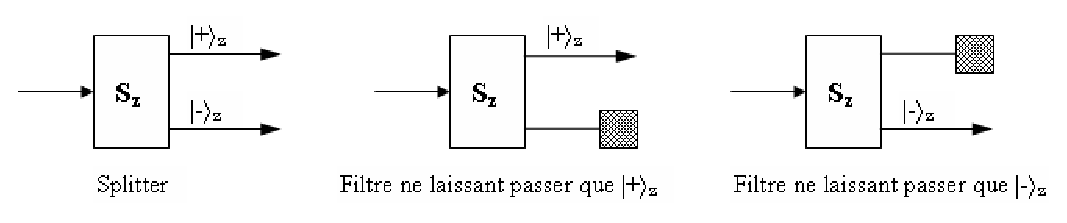
\includegraphics[scale=.9]{graphics/SGSplitterFiltre.eps}
\else
	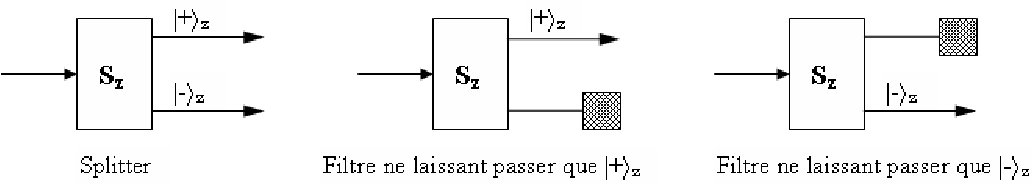
\includegraphics[scale=.9]{graphics/SGSplitterFiltre.pdf}
\fi
\caption{Stern et Gerlach comme séparateur du jet atomique ou splitter et comme
filtres.}%
\label{fig:SGsplitterFiltre}%
\end{figure}

Nous allons maintenant réaliser diverses expériences sur le spin en utilisant
les symboles de la figure \ref{fig:SGsplitterFiltre} pour les divers rôles des
appareils de Stern et Gerlach.

\subsubsection{Première expérience SG1}

A la sortie du filtre de la figure \ref{fig:sgszsz}, chaque atome est dans
un état propre de l'opérateur $S_{z}$ que l'on mesure. Le résultat de la
mesure est donc \textbf{certain}: on trouve à coup sûr la valeur propre
correspondante $+\frac{\hbar}{2}$%
\begin{equation}
\mathcal{P}(+\frac{\hbar}{2})=|\langle+\ket{+}|^{2}=1.
\end{equation}

\begin{figure}[ptbh]
\begin{minipage}[c]{.48\linewidth}
\centering
\ifcase\msipdfoutput
	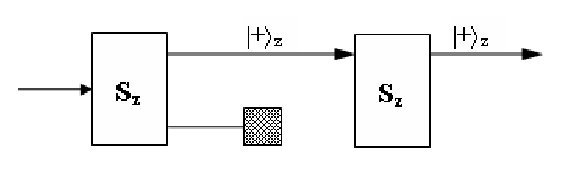
\includegraphics[scale=.8]{graphics/SGSzSz.eps}
\else
	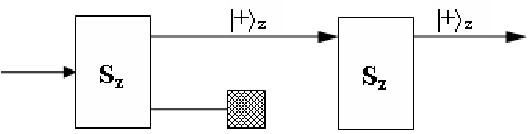
\includegraphics[scale=.8]{graphics/SGSzSz.pdf}
\fi
\caption{Mesure de $\mathcal{S}_{z}$ dans l'état $\ket{+}$.}%
\label{fig:sgszsz}%
\end{minipage} \hfill
\begin{minipage}[c]{.48\linewidth}
\centering
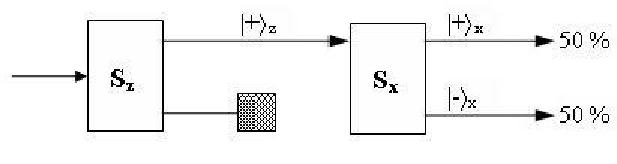
\includegraphics[scale=.8]{graphics/SGSzSx.pdf}
\caption{Mesure de $\mathcal{S}_{x}$ dans l'état $\ket{+}$.}%
\label{fig:sgszsx}%
\end{minipage}
\end{figure}


\subsubsection{Deuxième expérience SG2}

A la sortie du filtre de la figure \ref{fig:sgszsx}, chaque atome qui entre
dans le splitter orienté dans la direction $Ox$ est dans l'état $\ket{+}$. Lors
du processus de mesure de la grandeur $\mathcal{S}_{x}$, \textbf{il y a
indétermination dans le comportement de chaque atome} puisque $\ket{+}$
\emph{n'est pas un état propre de l'opérateur} $S_{x}$. Cet
opérateur à pour valeurs propres $+\frac{\hbar}{2}$ et $-\frac{\hbar}{2}$
associées respectivement aux états propres $\ket{+}_{x}$ et
$\ket{-}_{x}$. C'est parce que $\ket{+}$ se projette dans la base $\{
\ket{+}_{x},\ket{-}_{x}\}$ qui diagonalise $S_{x}$ qu'on observe à la sortie
deux faisceaux d'égales intensités, i.e.,

\begin{enumerate}
\item un faisceau où les atomes ont un spin $+\frac{\hbar}{2}$ avec la
probabilité $|_{x}\langle+\ket{+}|^{2}=\frac{1}{2}$;

\item un faisceau où les atomes ont un spin $-\frac{\hbar}{2}$ avec la
probabilité $|_{x}\langle-\ket{+}|^{2}=\frac{1}{2}$.
\end{enumerate}

\subsubsection{Troisième expérience SG3}

\begin{figure}[ptbh]
\centering
\ifcase\msipdfoutput
	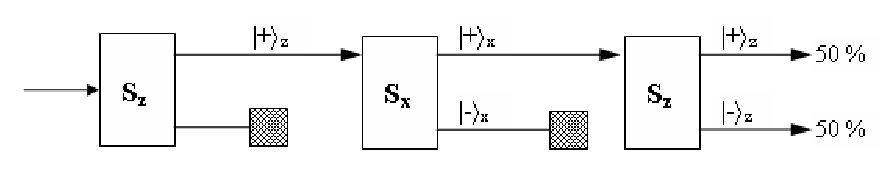
\includegraphics[scale=.9]{graphics/SGSzSxSzP.eps}
\else
	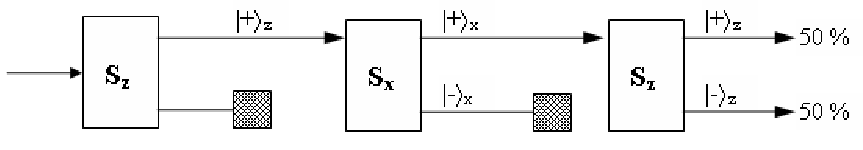
\includegraphics[scale=.9]{graphics/SGSzSxSzP.pdf}
\fi
\caption{Incompatibilité des mesures de $\mathcal{S}_{z}$ et $\mathcal{S}_{x}$.}
\label{fig:sgszsxszp}%
\end{figure}

On filtre maintenant $\ket{+}$ que fait pénétrer dans $S_{x}$. On filtre la
sortie de ce SG pour ne laisser sortir que $\ket{+}_{x}$ qui va pénétrer dans
un $S_{z}$. On constate avec surprise qu'on a à la sortie des atomes dans les
états propres $\ket{+}$ et $\ket{-}$ de $S_{z}$, alors que $\ket{-}$ a été
exclus à la sortie du premier SG, $S_{z}$.

Cette expérience met en exergue le fait qu'en théorie quantique, \emph{l'état
final du système dépend seulement de l'état de l'atome qui entre dans le dernier
SG et de son action avec cet appareil}. Autrement, il n'y a pas de mémoire sur
l'histoire passée du système.

En clair, comme le faisceau qui entre dans le dernier SG, $S_{z}$ est dans
l'état  $\ket{+}_{x}$ qui n'est pas état propre de $S_{z}$, il va se projeter
dans la base  \{$\ket{+},\ket{-}\}$ des états propres de $S_{z}$. C'est
pourquoi on a

\begin{enumerate}
\item un faisceau où les atomes ont un spin $+\frac{\hbar}{2}$ avec la
probabilité $|\langle+\ket{+}_{x}|^{2}=\frac{1}{2}$;

\item un faisceau où les atomes ont un spin $-\frac{\hbar}{2}$ avec la
probabilité $|\langle-\ket{+}_{x}|^{2}=\frac{1}{2}$.
\end{enumerate}

\subsection{Point sur la mesure}

Il découle de ce qui précède que:

\begin{enumerate}
\item L'acte de mesure modifie généralement d'une manière \emph{instantanée}
le système de façon \emph{irréversible}: c'est \textbf{la réduction du paquet
d'onde}.

\item \textbf{Le résultat complet de la mesure expérimentale} de la grandeur
physique $\mathcal{A}$ sur le système consiste à déterminer les modalités
$a_{i}$ (résultats de la mesure) et les amplitudes de probabilité $\alpha_{i}$
ou les probabilités $\mathcal{P}_{i}=|\alpha_{i}|^{2}$. Autrement dit, il s'agit
d'extraire des nombres contenus dans le vecteur d'état $\ket{\psi}$.

\item Les modalités $a_{i}$ dépendent de la \emph{nature} du système et les
amplitudes de probabilité $\alpha_{i}$ dépendent de l'\emph{état} du système
ou du vecteur d'état $\ket{\psi}$.

\item L'\textbf{opérateur} $A$ extrait de $\ket{\psi}$ l'information physique
sur la grandeur physique $\mathcal{A}$. $\ket{\psi}$ décrit la réalité physique
d'un système quantique individuel.

\item Lorsqu'on a \emph{un seul} système dans l'état $\ket{\psi}$, si \emph{une
seule} mesure de $\mathcal{A}$ donne la modalité $a_{i},$ le système est après
cette mesure dans l'état $\ket{\varphi_{i}}$ associé à $a_{i}$%
\begin{equation}
\ket{\varphi_{i}}=\ket{A\psi}=A\ket{\psi} ,
\end{equation}
$A$ est l'\emph{opérateur (hermitien)\footnote{Les propriétés d'un opérateur
hermitien sont étudiées à la \textbf{section} (\ref{sec:OOL})} associé à la
grandeur physique} $\mathcal{A}$. Si on répète cette mesure de $\mathcal{A}$
\textbf{immédiatement après }sur le système, qui est alors dans l'état
$\ket{\varphi_{i}}$, on obtiendra \emph{de façon certaine la même modalité}
$a_{i}$ \emph{avec la probabilité} $1$:%
\begin{subequations}%
\begin{align}
A\ket{\varphi_{i}} &  =a_{i}\ket{\varphi_{i}}\text{ ou }
A=\ket{\varphi_{i}}a_{i}\bra{\varphi_{i}} \\
\mathcal{P}(a_{i}) & =|\langle\varphi_{i}\ket{\varphi_{i}}|^{2}
=|\ket{\varphi_{i}}|^{2}=1.
\end{align}%
\end{subequations}%
Autrement dit, à chaque résultat possible $a_{i}$ de la mesure correspond un
état $\ket{\varphi_{i}}$ possédant la propriété ci-dessus, que nous appellerons
\textbf{état propre}\footnote{C'est un état simple qui peut être qualifié de
"\emph{déterministe}".} ou \textbf{vecteur propre} de l'opérateur $A$; $a_{i}$
est appelée \textbf{valeur propre} de l'opérateur $A$.

\medskip
\colorbox[gray]{0.8}{
\parbox[c]{0.9\textwidth}{
\emph{Donc, la \textbf{mesure de $\mathcal{A}$ sur un seul système} dans l'état
$\ket{\psi}$ donne l'information sur l'état du système \textbf{après la
mesure}}.
}}

\item Pour obtenir l'information sur l'état du système \textbf{avant la mesure}
il faut effectuer $N$\textbf{\ mesures} de $\mathcal{A}$ sur $N$
\textbf{systèmes identiques\footnote{On peut par exemple réaliser une expérience
de Stern et Gerlach avec $N$ voies de sorties au lieu de deux voies $\ket{+}$ et
$\ket{-}$ et un détecteur associé à chaque voie.}} dans l'état $\ket{\psi} $
afin d'obtenir toutes les modalités possibles $a_{i}$:%
\begin{subequations}
\begin{align}
\ket{\psi}  &  =\sum_{i}\ket{\varphi_{i}}\bra{\varphi_{i}}\ket{\psi}
=\sum_{i}\alpha_{i}\ket{\varphi_{i}},\label{eq:Proj1}\\
A\ket{\psi}  & =\sum_{i}\alpha_{i}A\ket{\varphi_{i}}
=\sum_{i}\alpha_{i}a_{i}\ket{\varphi_{i}}.
\end{align}%
\end{subequations}%
L'ensemble des états propres $\ket{\varphi_{i}}$ de la grandeur physique forme
une base orthonormée
\begin{equation}
\langle\varphi_{i}\ket{\varphi_{j}}=\begin{cases}
1, & \text{si }i=j.\\
0, & \text{sinon.}%
\end{cases}
\end{equation}
D'où les propriétés suivantes de leurs probabilités de transition%
\begin{equation}%
\begin{array}
[c]{cccc}%
\mathcal{P}(\langle\varphi_{i}\ket{\varphi_{j}})=0, & \forall i,j &
i\neq j & \text{(\textbf{disjonction),}}\\
&  &  & \\
\sum_{i}\mathcal{P}(\langle\varphi_{i}\ket{\psi})=1, & \forall\ket{\psi}  &  &
\text{(\textbf{complétude).}}%
\end{array}
\end{equation}
\end{enumerate}


\section{Opérateurs linéaires et représentation matricielle}
\label{sec:OOL}

\colorbox[gray]{0.8}{
\parbox[c]{0.9\textwidth}{
\begin{principe}
A chaque grandeur physique $\mathcal{A}$, l'on peut associer un
\textbf{opérateur} $A$, \textbf{qui est linéaire hermitien} agissant dans
l'espace de Hilbert $\mathcal{H}$, tel que la valeur moyenne $\langle a\rangle
_{\psi}$ des résultats d'une mesure de la grandeur $\mathcal{A}$ pour un
quanton dans l'état $\ket{\psi}$ soit%
\begin{equation}
\langle a\rangle =\bra{\psi}A\ket{\psi}.
\end{equation}
\end{principe}
}}\medskip

Les opérateurs de la théorie quantique sont linéaires et cette linéarité est
intimement lié au \textbf{principe de superposition}.

\subsection{Linéarité et représentation matricielle}

On appelle \textbf{opérateur linéaire }$A$ de $\mathcal{H}$, toute
application linéaire
\begin{equation}%
\begin{array}
[c]{ccll}%
A: & \mathcal{H} & \longrightarrow & \mathcal{H}\\
& \ket{\psi}  & \longrightarrow & \ket{\varphi} =\ket{A\psi} \equiv A\ket{\psi}
\end{array}
\end{equation}
vérifiant la propriété
\begin{equation}
\ket{A(\lambda_1\psi_1+\lambda_{2}\psi_{2})}
=\lambda_1\ket{A\psi_1} +\lambda_{2}\ket{A\psi_{2}}
=\lambda_1\ket{\varphi_1} +\lambda_{2}\ket{\varphi_{2}}.
\end{equation}
Un exemple simple d'opérateur linéaire est l'opérateur identité $\mathbb{I}$:%
\begin{equation}
\ket{\mathbb{I}\psi} =\ket{\psi}.
\end{equation}

L'algèbre sur ces opérateurs est la suivante,
\begin{subequations}%
\begin{align}
\ket{(\lambda A)\psi} &  =\lambda\ket{A\psi},\\
\ket{(A+B)\psi} &  =\ket{A\psi} +\ket{B\psi},\\
\ket{(AB)\psi} &  =\ket{A(B\psi)}.
\end{align}%
\end{subequations}%

Afin de déterminer l'effet de l'opérateur linéaire $A$ sur n'importe quel état
$\ket{\psi}$ dans une base $\{\ket{i}\}$, utilisons la décomposition
(\ref{eq:Proj1})
\begin{equation}
\begin{cases}
\ket{\varphi} =A\ket{\psi}=\sum_{i}\ket{i}\bra{i} A\ket{\psi},\\
\ket{\psi}=\sum_{j}\ket{j}\langle j\ket{\psi},
\end{cases}  \Rightarrow\ket{\varphi} =\sum_{i,j}\ket{i}\bra{i}A\ket{j}\langle
j\ket{\psi}. \label{Jii}%
\end{equation}

Il apparaît ainsi que si l'on connaît les \textbf{matrices d'amplitudes}
ou \textbf{éléments de matrice}%
\begin{equation}
A_{ij}=\bra{i} A\ket{j}=\langle i\ket{Aj},
\label{iAj}%
\end{equation}
entre tous les états $\{\ket{i}\}$ de cette base, on peut déterminer
l'effet de l'opérateur $A$ sur n'importe quel état $\ket{\psi}$.

Si la base $\{\ket{i}\}$ à $n$ états, alors les amplitudes $(n\times n)$ de
l'équation (\ref{iAj}) définissent complètement l'opérateur $A$.

\medskip\colorbox[gray]{0.8}{
\parbox[c]{0.9\textwidth}{
\emph{Les opérateurs sont donc définis par les matrices d'amplitudes $(n\times
n) $ dans une représentation particulière}%
\begin{equation}
A\longrightarrow\bra{i} A\ket{j} =\langle i\ket{Aj} =A_{ij}\Longleftrightarrow%
\begin{array}
[c]{c}%
\ket{Aj} \longrightarrow\\
\bra{i} \downarrow\begin{pmatrix}
A_{11} & A_{12} & \cdots & A_{1j} & \cdots\\
A_{21} & A_{22} & \cdots & A_{2j} & \cdots\\
\vdots & \vdots &  &  & \\
A_{i1} & A_{i2} & \cdots & A_{ij} & \cdots\\
\vdots & \vdots &  & \vdots &
\end{pmatrix}
\end{array}
.
\end{equation}
}}
\medskip

Les amplitudes dans une matrice définissant l'opérateur $A$ dépendent de la
représentation. La transformation des éléments de matrices lors d'un changement
de base est
\begin{equation}
\bra{\nu}A\ket{\mu} =\sum_{ij}\langle \nu\ket{i}\bra{i}A\ket{j}\langle j
\ket{\mu},
\end{equation}
où $\langle\nu\ket{i}$ et $\langle j\ket{\mu}$ sont les éléments de la
transformation de la base $\{\ket{i}\}$ à la base $\{\ket{\mu}\}$ et
vice-versa.

\begin{example}
Soient les opérateurs $X=\sqrt{\alpha}x$ et $P=\frac{1}{\sqrt{\alpha}}\frac
{d}{dx}$. L'action des opérateurs $x$ et $\frac{d}{dx}$ sur les états
$\ket{n}$ d'un oscillateur harmonique donne les fonctions
d'Hermite suivantes:
\begin{subequations}%
\begin{gather}
\sqrt{2\alpha}x\ket{n}=\sqrt{n+1}\ket{n+1}+\sqrt{n}\ket{n-1},\\
\sqrt{\frac{2}{\alpha}}\frac{d}{dx}\ket{n}=-\sqrt{n+1}\ket{n+1}+\sqrt{n}\ket{n-1
}.
\end{gather}%
\end{subequations}%
Les matrices des opérateurs $X$ et $P$ sur les états $\ket{n}$ sont%
\begin{equation}
\begin{split}
X_{mn}  &  =\bra{m}X\ket{n}=\frac{1}{\sqrt{2}}\bra{m}\sqrt{2\alpha}x\ket{n}\\
&  =\frac{1}{\sqrt{2}}(\sqrt{n+1}\langle m\ket{n+1}+\sqrt{n}\langle m \ket{n-1})
\\
&=\frac{1}{\sqrt{2}}(\sqrt{n+1}\delta_{m,n+1}+\sqrt{n}\delta_{m,n-1}),
\end{split}
\end{equation}
et%
\begin{equation}
\begin{split}
P_{mn}  &  =\bra{m}P\ket{n}=\frac{1}{\sqrt{2}}\bra{m}\sqrt{\frac{2}{\alpha}}
\frac{d}{dx}\ket{n}\\
&  =\frac{1}{\sqrt{2}}(-\sqrt{n+1}\langle m\ket{n+1}+\sqrt{n}\langle m\ket{n-1})
\\
&
=\frac{1}{\sqrt{2}}(-\sqrt{n+1}\delta_{m,n+1}+\sqrt{n}\delta_{m,n-1}).
\end{split}
\end{equation}
Pour $n,m\in[0,3]$ on a les représentations matricielles du tableau
\ref{tab:matrXP}.%

\begin{table}[htbp] \centering
\begin{tabular}
[c]{l|llll}\cline{1-1}%
\multicolumn{1}{|l|}{$X_{mn}$} & \cellcolor[gray]{.8}$\ket{X0}$ &
\cellcolor[gray]{.8}$\ket{X1}$ &
\cellcolor[gray]{.8}$\ket{X2}$ &
\cellcolor[gray]{.8}$\ket{X3}$\\\hline
\cellcolor[gray]{.8}$\bra{0}$ & $0$ &
\multicolumn{1}{|l}{$\frac{1}{\sqrt{2}}$} & \multicolumn{1}{|l}{$0$} &
\multicolumn{1}{|l|}{$0$}\\\cline{2-5}%
\cellcolor[gray]{.8}$\bra{1}$ & $\frac{1}{\sqrt{2}}$ &
\multicolumn{1}{|l}{$0$} & \multicolumn{1}{|l}{$1$} & \multicolumn{1}{|l|}{$0$%
}\\\cline{2-5}%
\cellcolor[gray]{.8}$\bra{2}$ & $0$ &
\multicolumn{1}{|l}{$1$} & \multicolumn{1}{|l}{$0$} &
\multicolumn{1}{|l|}{$\sqrt{\frac{3}{2}}$}\\\cline{2-5}%
\cellcolor[gray]{.8}$\bra{3}$ & $0$ &
\multicolumn{1}{|l}{$0$} & \multicolumn{1}{|l}{$\sqrt{\frac{3}{2}}$} &
\multicolumn{1}{|l|}{$0$}\\\cline{2-5}%
\end{tabular}
\begin{tabular}
[c]{l|llll}\cline{1-1}%
\multicolumn{1}{|l|}{$P_{mn}$} & \cellcolor[gray]{.8}$\ket{
P0}$ & \cellcolor[gray]{.8}$\ket{P1}$ &
\cellcolor[gray]{.8}$\ket{P2}$ &
\cellcolor[gray]{.8}$\ket{P3}$\\\hline
\cellcolor[gray]{.8}$\bra{0}$ & $0$ &
\multicolumn{1}{|l}{$\frac{1}{\sqrt{2}}$} & \multicolumn{1}{|l}{$0$} &
\multicolumn{1}{|l|}{$0$}\\\cline{2-5}%
\cellcolor[gray]{.8}$\bra{1}$ & $-\frac{1}{\sqrt{2}}$ &
\multicolumn{1}{|l}{$0$} & \multicolumn{1}{|l}{$1$} & \multicolumn{1}{|l|}{$0$%
}\\\cline{2-5}%
\cellcolor[gray]{.8}$\bra{2}$ & $0$ &
\multicolumn{1}{|l}{$-1$} & \multicolumn{1}{|l}{$0$} &
\multicolumn{1}{|l|}{$\sqrt{\frac{3}{2}}$}\\\cline{2-5}%
\cellcolor[gray]{.8}$\bra{3}$ & $0$ &
\multicolumn{1}{|l}{$0$} & \multicolumn{1}{|l}{$-\sqrt{\frac{3}{2}}$} &
\multicolumn{1}{|l|}{$0$}\\\cline{2-5}%
\end{tabular}
\caption{Matrices des opérateurs $X$ et $P$ sur les états $\ket{n}$ d'un
oscillateur harmonique.}\label{tab:matrXP}%
\end{table}%

\end{example}

\subsection{Hermiticité et fonction d'un opérateur}

\label{sec:HermFctOp}

L'opérateur \textbf{adjoint} ou \textbf{hermitien conjugué} $A^{\dagger}$ de
$A$ est défini par%
\begin{equation}
\bra{\varphi}A^{\dagger}\psi\rangle =\langle A\varphi\ket{\psi}
=\bra{\psi}A\varphi\rangle^{\ast}\text{, }\ket{\psi},\ket{\varphi}
\in\mathcal{H}.
\end{equation}

On montre facilement que %
\begin{subequations}%
\begin{align}
(A^{\dagger})^{\dagger}=A,\\
(\lambda A+\mu B) ^{\dagger}=\lambda^{\ast}A^{\dagger}+\mu^{\ast}B^{\dagger},\\
(AB)^{\dagger}=B^{\dagger}A^{\dagger}.
\end{align}%
\end{subequations}%

\medskip
\colorbox[gray]{0.8}{
\parbox[c]{0.9\textwidth}{
\emph{\textbf{Algorithme pour prendre le conjugué hermitien} d'une
expression donnée:}

\begin{enumerate}
\item \emph{renverser l'ordre des termes};

\item \emph{remplacer}

\begin{enumerate}
\item \emph{les opérateurs par leurs adjoints};

\item \emph{les kets par les bras et réciproquement};

\item \emph{les nombres par leurs complexes conjugués}.%
\end{enumerate}
\end{enumerate}
}}

\begin{example}

\begin{equation}
(\lambda\bra{\varphi}AB\ket{\psi}\bra{\chi}C^{\dagger})^{\dagger}=C\ket{\chi}
\bra{\psi}B^{\dagger}A^{\dagger}\ket{\varphi} \lambda^{\ast}.
\end{equation}
\begin{equation}
(2\ket{0}\bra{1}-i\ket{1}\bra{0})^{\dag}=+i\ket{0}\bra{1}+\ket{1}\bra{0}2.
\end{equation}
Pas du tout compliqué n'est-ce pas?!!!!
\end{example}

Dans la base $\{\ket{i}\}$, l'opérateur adjoint $A^{\dag}$ vérifie%
\begin{equation}
(A^{\dag})_{ij}=A_{ji}^{\ast}=(A_{ij}^{t})^{\ast}\Rightarrow A^{\dag}
=(A^{t})^{\ast}.
\end{equation}

Ainsi, les matrices représentant $A$ et $A^{\dag}$ dans une représentation
sont hermitiennes conjuguées l'une de l'autre, au sens des matrices: \emph{on
passe de l'une à l'autre par une conjugaison complexe suivie d'une symétrie
par rapport à la diagonale principale. }

Il va de soi que lorsque $A$ est une matrice réelle, $A^{\dag}=A^{t}$.
\begin{example}%
\begin{subequations}%
\begin{align}
\begin{pmatrix}
2+i & -i\\
4-i & 2+i
\end{pmatrix} ^{\dag}  &  =\begin{pmatrix}
2-i & 4+i\\
i & 2-i
\end{pmatrix} ;\\
\begin{pmatrix}
i & 2+i\\
4i & 3-2i
\end{pmatrix} ^{\dag}  &  =\allowbreak\begin{pmatrix}
-i & -4i\\
2-i & 3+2i
\end{pmatrix} ;\\
\begin{pmatrix}
a+ib & c+id\\
e+if & g+ih
\end{pmatrix} ^{\dag}  &  =\allowbreak\begin{pmatrix}
a-ib & e-if\\
c-id & g-ih%
\end{pmatrix} ;\\
\begin{bmatrix}
-85 & -55 & -37\\
-35 & 97 & 50\\
79 & 56 & 49
\end{bmatrix}^{\dag}  &  =\begin{bmatrix}
-85 & -35 & 79\\
-55 & 97 & 56\\
-37 & 50 & 49
\end{bmatrix}.
\end{align}
\end{subequations}%

\end{example}

Un opérateur $A$ est \textbf{hermitien }ou \textbf{auto-adjoint}, s'il
coïncide avec son adjoint:%
\begin{equation}
A^{\dagger}=A.
\end{equation}
Par conséquent%
\begin{equation}
\begin{cases}
A_{ij}^{\dag}=A_{ij}=A_{ji}^{\ast}\text{ si }i\neq j,\\
A_{ii}^{\dag}=A_{ii}=A_{ii}^{\ast}.
\end{cases}
\end{equation}


\colorbox[gray]{0.8}{
\parbox[c]{0.9\textwidth}{
Ainsi, dans une matrice hermitienne

\begin{enumerate}
\item \emph{deux éléments quelconques symétriques par rapport à la diagonale
principale sont complexes conjugués l'un de l'autre,}

\item \emph{les éléments diagonaux sont toujours réels.}
\end{enumerate}
}}\medskip

Ceci nous permet de comprendre aisément pourquoi Zurek affirme que \emph{la
réalité serait quantique mais aurait une apparence classique par le fait que les
éléments non diagonaux sont très petits et leurs effets inobservables de façon
pratique.}

La forme générale d'une matrice hermitienne $2\times2$ est%
\begin{equation}
\begin{pmatrix}
a_{11} & a_{12}\\
a_{12}^{\ast} & a_{22}%
\end{pmatrix} ,
\end{equation}
où $a_{11}$, $a_{22}\in\mathbb{R}$ et $a_{12}$ \emph{à priori} complexe.

\emph{\textbf{Les opérateurs de la théorie quantique sont hermitiens.}} Les
importantes conséquences sur leurs spectres seront étudiées à la
\textbf{section \ref{sec:DSO}}.

\textbf{La fonction d'un opérateur} $f(A)$ peut être développée
comme une série entière%

\begin{equation}
f(A)=\sum_{n}^{\infty}c_{n}A^{n}.
\end{equation}

Par exemple,
\begin{equation}
e^{A}=\mathbb{I}+A+\frac{1}{2}A^{2}+\ldots+\frac{1}{n!}A^{n}+\ldots
\end{equation}

\colorbox[gray]{0.8}{
\parbox[c]{0.9\textwidth}{
\emph{Si $\ket{\psi}$ est vecteur propre de $A$ avec la valeur propre $a$,
$\ket{\psi}$ est aussi vecteur propre de $f(A)$ avec la valeur propre $f(a)$}

\begin{equation}
f(A)\ket{\psi}=\sum_{n}^{\infty}c_{n}%
A^{n}\ket{\psi}=\sum_{n}^{\infty}c_{n}a^{n}\ket{\psi}=f(a)\ket{\psi}.
\end{equation}
}}

\begin{example}
Pour $A=\begin{pmatrix}1 & 0\\0 & -1\end{pmatrix} $, on a l'opérateur
$e^A=\begin{pmatrix}e^{1} & 0\\0 & e^{-1}\end{pmatrix}$.

Pour $B=\begin{pmatrix}0 & 1\\1 & 0\end{pmatrix},$ on a pour tout entier $n$,
$B^{2n}=\mathbb{I}_{2}$, la matrice unité de rang $2$, et $B^{2n+1}=B$, et par
conséquent,
\begin{equation}
\label{eq:ExpoB}
\begin{split}
e^{i\alpha B} &  =\sum_{n=0}^{\infty}\frac{(i\alpha B)^{2n}}{(2n)!}
+\sum_{n=0}^{\infty}\frac{(i\alpha B)^{2n+1}}{(2n+1)!}
=\mathbb{I}_{2}\sum_{n=0}^{\infty}\frac{(i\alpha)^{2n}}{(2n)!}+B\sum_{n=0}%
^{\infty}\frac{(i\alpha)^{2n+1}}{(2n+1)!}\\
&  =(\cos\alpha)\mathbb{I}_{2}+i(\sin\alpha)B.
\end{split}
\end{equation}

\end{example}

Si les $a_{i}$ sont les valeurs propres de l'opérateur $A$ dans la base
$\{\ket{\varphi_{i}}\}$, la \textbf{trace} de cet opérateur est la somme de ses
éléments diagonaux
\begin{equation}
\opn{tr}A=\sum_{i}\bra{\varphi_{i}} A\ket{\varphi_{i}} 
=\sum_{i}a_{i}=\sum_{i}A_{ii}.
\end{equation}
La trace est invariante dans un changement de base et on a
\begin{equation}%
\begin{array}{ll}
\opn{tr}(A+B) =\opn{tr}A+\opn{tr}B, &
\text{(linéarité),}\\
\opn{tr}(cA) =c\opn{tr}A, & (c\in\mathbb{C})\\
\opn{tr}AB =\opn{tr}BA, & \text{(propriété cyclique).}
\end{array}
\end{equation}

\begin{example}
 Dans la base $\{\ket{0},\ket{1}\}$, la trace de l'opérateur
\begin{subequations}
\begin{align}
 A=2i\ket{0}\bra{0}+3\ket{0}\bra{1}-2\ket{1}\bra{0}+4\ket{1}\bra{1}
\end{align}
est
\begin{align}
\opn{tr}(A)=\bra{0}A\ket{0}+\bra{1}A\ket{1}=2i+4.
\end{align}
\end{subequations}
\end{example}

\subsection{Unitarité}

Un opérateur $S$ est dit \textbf{unitaire} s'il est l'inverse de son adjoint,
i.e.,
\begin{equation}
S^{\dag}=S^{-1}\text{, i.e.,} SS^{\dagger}=S^{\dagger}S=\mathbb{I},
\end{equation}
et par conséquent \emph{\textbf{conserve la norme}} de tout vecteur d'état,
\begin{equation}
\|S\ket{\psi}\|^2 =\bra{\psi}S^{\dagger}S\ket{\psi}=\|\ket{\psi}\|^2.
\end{equation}

\begin{proof}
Si $\ket{\psi_{i}}$ et $\ket{\varphi_{i}}$ sont deux bases orthonormées
complètes, et si
\begin{equation}
S\ket{\psi_{i}}=\ket{\varphi_{i}},
\end{equation}
alors
\begin{equation}
S=S\mathbb{I}=S\sum_{i}\ket{\psi_{i}}\bra{\psi_{i}}=\sum_{i}\ket{\varphi_{i}}
\bra{\psi_{i}},
\end{equation}
et
\begin{equation}
S^{\dagger}=\sum_{i}\ket{\psi_{i}}\bra{\varphi_{i}}.
\end{equation}
Et par suite,
\begin{equation}
SS^{\dagger}=\sum_{i,j}\ket{\varphi_{i}}\langle\psi_{i}\ket{\psi_{j}}
\bra{\varphi_{j}}=\sum_{i,j}\ket{\varphi_{i}}\delta_{ij}\bra{\varphi_{j}}
=\mathbb{I}.
\end{equation}

\end{proof}

On peut construire des opérateurs unitaires par exponentiation d'opérateurs
hermitiens $A$%
\begin{equation}
S(\lambda)=e^{-i\lambda A},
\label{eq:Sexp}%
\end{equation}
avec $\lambda$ une paramètre continu réel. De plus, $S(\lambda)
$ vérifie la propriété de groupe abélien%
\begin{subequations}%
\begin{align}
S(\lambda_1+\lambda_{2}) &  =S(\lambda_1)S(\lambda_{2}),\\
S(0) &  =\mathbb{I}.
\end{align}%
\end{subequations}%
La réciproque de cette propriété est le théorème de Stone.

\medskip
\colorbox[gray]{0.8}{
\parbox[c]{0.9\textwidth}{
\begin{theorem}
\label{Th:stone} \textbf{Stone.} Soit un ensemble d'opérateurs unitaires
dépendant d'un paramètre continu $\lambda$ et vérifiant la loi du groupe
abélien. Il existe alors un opérateur hermitien $G$, appelé \textbf{générateur
infinitésimal} du groupe de transformations $S(\lambda)$ tel que $S(\lambda)
=e^{-i\lambda G}$.
\end{theorem}
}}
\medskip

\begin{proof}
Si $\delta\lambda\rightarrow0$,
\begin{equation}
S(\lambda+\delta\lambda)=S(\lambda)S(\delta\lambda)\simeq(\mathbb{I}
-i\delta\lambda B)S(\lambda),
\end{equation}
avec%
\begin{equation}
B=i\left\vert \frac{dS}{d\lambda}\right.  _{\lambda=0}.
\end{equation}
Alors%
\begin{equation}
\frac{dS(\lambda)}{d\lambda}=-iBS(\lambda).
\end{equation}
Par intégration on trouve, en tenant compte de $S(0)=\mathbb{I}$ et en
posant$G=B$, $S(\lambda)=e^{-i\lambda G}$.
\end{proof}

Un opérateur $A$ est une \textbf{isométrie} si
\begin{equation}
A^{\dag}A=\mathbb{I},
\end{equation}
puisque le produit scalaire est préservé%
\begin{equation}
\bra{\varphi A^{\dag}} A\psi\rangle= \langle\varphi\ket{\psi}.
\end{equation}

Il est à noter qu'il existe des opérateurs isométriques non unitaire ou
anti-unitaire.

\subsection{Projection}

Une classe importante des opérateurs linéaires hermitiens est celle des
\textbf{opérateurs projecteurs} $P$ caractérisés par les propriétés de
normalisation, d'orthogonalité et d'hermiticité suivantes

\medskip
\colorbox[gray]{0.8}{
\parbox[c]{0.9\textwidth}{
\begin{subequations}
\begin{align}
P_{i}^{2} & = P_{i},\\
P_{i}P_{j}  &  =\delta_{ij}P_{i},\\
P_{i}^{\dagger}  &  =P_{i}.
\end{align}
\end{subequations}
}}\medskip

L'opérateur projecteur
\begin{equation}
P_{i}=\sum_{i=1}^{m\leq n}\ket{i}\bra{i},
\label{Oproj2}
\end{equation}
projette l'état $\ket{\psi}$ sur la base orthonormée $\{\ket{i}\} $ de dimension
$m$ du sous-espace $\mathcal{H}^{\prime}$ de $\mathcal{H}$ (qui est de dimension
$n$):
\begin{equation}
P_{i}\ket{\psi}=\sum_{i}\ket{i}\bra{i}\psi\rangle=\sum_{i}\langle i\ket{\psi}
\ket{i}=\sum_{i}\alpha_{i}\ket{i}.
\end{equation}
On montre facilement que $P_{i}$ est hermitien%
\begin{equation}
P_{i}^{\dagger}=(\sum_{i}\ket{i}\bra{i})^{\dagger}=\sum_{i}\ket{i}\bra{i}=P_{i},
\end{equation}
et qu'il vérifie la relation de normalisation
\begin{equation}
P_{i}^{2}=\sum_{i}\ket{i}\langle i\ket{i}\bra{i}=\sum_{i}\ket{i}\bra{i} =P_{i}.
\end{equation}
Les seules valeurs propres d'un opérateur projecteur sont $0$ et $1$. En effet,
si $\ket{p}$ est vecteur propre de l'opérateur $P$ avec la valeur propre $p$,
$P\ket{p}=p\ket{p}$, la condition nécessaire et suffisante $P^{2}=P$ entraîne%
\begin{equation}
P^{2}\ket{p}-P\ket{p}=0\Rightarrow p^{2}-p=p(p-1)=0\text{, i.e., }p=0\text{ ou
}p=1.
\end{equation}

Lorsque $m=n$ dans l'équation (\ref{Oproj2}), on obtient la décomposition de
l'opérateur \textbf{identité} $\mathbb{I}$
\begin{equation}
\mathbb{I}=\sum_{i=1}^{n}\ket{i}\bra{i} .
\end{equation}
C'est la \textbf{\emph{relation de fermeture}}. Elle exprime le fait que
l'ensemble $\{\ket{i}\}$ est une base hilbertienne.

\section{Décomposition spectrale des opérateurs hermitiens}

\label{sec:DSO}

Comme nous l'avons vu à la \textbf{section \ref{sec:HermFctOp}}, les opérateurs
de théorie quantique associés aux grandeurs physiques sont hermitiens.
\textbf{\emph{Leur spectre est par conséquent réel et l'ensemble de leurs
vecteurs propres est complet.}} Certains opérateurs, comme par exemple
l'hamiltonien de l'oscillateur harmonique, ont un spectre discret. \emph{Il est
alors possible de construire une base hilbertienne à partir de l'ensemble de
leurs vecteurs propres}.

L'étude de ces propriétés importantes des opérateurs hermitiens est l'objet de
cette section.

\subsection{Diagonalisation d'un opérateur hermitien}

Un vecteur $\ket{\psi}$ est dit \textbf{vecteur propre} \textbf{de} $A$ si
\begin{equation}
A\ket{\psi}=a\ket{\psi},
\label{EVP}
\end{equation}
le nombre $a$ étant la \textbf{valeur propre} associée à ce vecteur propre.

\begin{enumerate}
\item Lorsqu'il correspond à $a$ un vecteur propre unique à un facteur
multiplicatif près, on dit que $a$ est \textbf{non-dégénéré}. \textbf{Tous les
vecteurs d'état associés sont colinéaires}.

\item Si au contraire, il existe plusieurs kets indépendants qui soient
vecteurs propres de $A$, $a$ est dit \textbf{dégénéré}. Son \emph{degré de
dégénérescence} est le nombre de vecteurs propres linéairement indépendant qui
lui sont associés.
\end{enumerate}

On appelle \textbf{spectre} d'un opérateur $A$, l'ensemble de ses valeurs
propres. On obtient ses valeurs propres en résolvant l'équation (\ref{EVP}): on
dit qu'on \textbf{\emph{diagonalise}} la matrice représentant $A$. Les éléments
diagonaux de cette matrice diagonale sont les valeurs propres.

\medskip
\colorbox[gray]{0.8}{
\parbox[c]{0.9\textwidth}{
\emph{\textbf{L'algorithme pour la diagonalisation} explicite d'une
matrice hermitienne $A$ de dimension finie $n$ est la suivante:}

\begin{enumerate}
\item Résoudre \emph{l'équation caractéristique ou séculaire $\det(A-\lambda
\mathbb{I})=0$ afin de trouver les $n$ valeurs propres $\lambda$ de $A$.}

\item \emph{Résoudre $A_{ij}\alpha_{j}=\lambda\alpha_{i}$ ($A\ket{\psi}
=\lambda\ket{\psi}$) pour chaque vecteur propre de $A$ (les $\alpha_{i}$ sont
les composantes ou amplitudes de projection de ces vecteurs propres de $A$). Ce
qui revient à résoudre un système de $n$ équations à $n$ inconnues.}
\end{enumerate}
}}
\medskip

\textbf{\emph{L'ensemble des vecteurs propres $\{\ket{\varphi_{i}}\}$ d'un
opérateur hermitien $A$ forme une base orthonormée dans $\mathcal{H}$.}}

Dans un espace de Hilbert fini $\mathcal{H}$, lorsque les valeurs propres
$a_{i}$ sont \emph{non-dégénérées}
\begin{equation}
A\ket{\varphi_{i}}=a_{i}\ket{\varphi_{i}},
\end{equation}
la \textbf{décomposition spectrale }de la matrice hermitienne $A$ est%
\begin{equation}
A=\sum_{i}a_{i}P_{i}=\sum_{i}a_{i}\ket{\varphi_{i}}\bra{\varphi_{i}}
=\sum_{i}\ket{\varphi_{i}}a_{i}\bra{\varphi_{i}}.
\label{DecSpec}
\end{equation}
Des équations (\ref{eq:Proj1}) et (\ref{DecSpec}) il apparaît que
l'\emph{opérateur projecteur}
\begin{equation}
P_{i}=\ket{\varphi_{i}}\bra{\varphi_{i}},
\label{OpProj}%
\end{equation}
permet soit

\begin{enumerate}
\item \textbf{de faire passer un test} $\ket{\varphi_{i}}$ à un système
quantique (Eq.(\ref{eq:Proj1})) lorsqu'on est intéressé par la probabilité de
trouver le système dans un \emph{état propre} de l'opérateur $A$: la mesure de
$P_{i}$ vaut $1$ si le test réussi et vaut $0$ si le test échoue;

\item \textbf{de mesurer la grandeur physique} $\mathcal{A}$ lorsqu'on est
plutôt intéressé par une valeur propre $a_{i}$ de l'opérateur $A$.
\end{enumerate}

Par exemple, lors de la mesure de la composante suivant $Oz$ du spin avec
l'appareil de Stern et Gerlach, on obtient les valeurs $\pm\frac{\hbar}{2}$ de
la grandeur physique $\mathcal{S}_{z}$. On peut aussi dire qu'on fait passer
aux atomes le test $\ket{+}$ et $\ket{-}$ avec les probabilités respectives
$|\langle +\ket{\psi}|^{2}$ et $|\langle -\ket{\psi}|^{2}$ de déviations vers le
haut et vers le bas.

\begin{remark}
Dans une mesure idéale ou un test idéal, on suppose que le système physique
n'est pas détruite par la mesure. Lorsqu'on répète plusieurs fois une même
mesure idéale, on a \textbf{mesure quantique sans démolition} ou mesure
Quantum Non Demolition (QND).
\end{remark}

\colorbox[gray]{0.8}{
\parbox[c]{0.9\textwidth}{
\begin{theorem}
\label{pr:VOrth} Les valeurs propres d'un opérateur hermitien sont réelles et
les vecteurs propres d'un opérateur hermitien correspondants à deux valeurs
propres différentes sont orthogonaux.
\end{theorem}
}}\medskip

\begin{proof}
\begin{align}
A  &  =A^{\dagger}\Rightarrow\bra{\varphi_{i}}A\ket{\varphi_{i}}
=\bra{\varphi_{i}}A^{\dagger}\ket{\varphi_{i}}
=\bra{\varphi_{i}}A\ket{\varphi_{i}}^{\ast}.\nonumber\\
\text{Si }A\ket{\varphi_{i}}  &  =a_{i}\ket{\varphi_{i}},
\text{ alors }
\begin{cases}
\bra{\varphi_{i}}A\ket{\varphi_{i}}=a_{i},\\
\bra{\varphi_{i}}A\ket{\varphi_{i}}^{\ast}=a_{i}^{\ast},
\end{cases}
\Rightarrow a_{i}=a_{i}^{\ast}\text{, i.e., }a_{i}\in\mathbb{R}.
\end{align}

D'autre part,
\begin{subequations}%
\begin{align}
\begin{cases}
A\ket{\varphi_{i}} =a_{i}\ket{\varphi_{i}},\\
A\ket{\varphi_{j}} =a_{j}\ket{\varphi_{j}},\\
a_{i}\neq a_{j},
\end{cases}
&  \Rightarrow
\begin{cases}
\bra{\varphi_{j}}A\ket{\varphi_{i}}=a_{i}\langle\varphi\ket{\varphi_{i}},\\
\bra{\varphi_{j}}A\ket{\varphi_{i}}=a_{j}\langle\varphi_{j}\ket{\varphi_{i}},
\end{cases}\\
&  \Rightarrow(a_{i}-a_{j})\langle\varphi_{j}\ket{\varphi_{i}}=0,\\
&  \Rightarrow\langle\varphi_{j}\ket{\varphi_{i}} =0\text{, puisque par
hypothèse }a_{i}\neq a_{j}.\nonumber\\
&  \Rightarrow\langle\varphi_{j}\ket{\varphi_{i}}=\delta_{ij}.
\end{align}%
\end{subequations}
\end{proof}

\textbf{\emph{Par conséquent, les vecteurs propres normalisés à l'unité d'un
opérateur hermitien forment une base orthonormée de $\mathcal{H}$ lorsque toutes
les valeurs propres sont différentes.}} Physiquement, cela entraîne que toute
amplitude peut être décomposée suivant les amplitudes qui sont les projections
des vecteurs propres de la grandeurs physique (donc suivant les amplitudes de
base). Le principe de superposition des états est donc lié au caractère
mathématique fermé du systèmes des vecteurs propres d'un opérateur hermitien.

\colorbox[gray]{0.8}{
\parbox[c]{0.9\textwidth}{
\begin{theorem}
Si un opérateur $A$ est hermitien, il est toujours possible de trouver un
matrice unitaire $S$ (non unique) telle que $S^{-1}AS$ soit une matrice
diagonale, dont les éléments diagonaux sont les valeurs propres qui apparaissent
sur la diagonale un nombre de fois égal à leur dégénérescence.

\begin{equation}
S^{-1}AS=\begin{pmatrix}
a_1 & 0 & 0 & \cdots & 0\\
0 & a_{2} & 0 & \cdots & \vdots\\
0 & 0 & a_3 & 0 & \vdots\\
\vdots& \vdots &  \ddots&  \ddots& 0\\
0 & \cdots & \cdots & 0 & a_{n}
\end{pmatrix}
\end{equation}
\end{theorem}
}}\medskip

\begin{example}
On considère la matrice
\begin{equation}
H=\begin{pmatrix}
0 & 1 & 0\\
1 & 0 & 1\\
0 & 1 & 0
\end{pmatrix} .
\end{equation}
Les valeurs propres de cette matrice déterminées par l'équation caractéristique%
\begin{equation}
\det(H-\lambda\mathbb{I})=\det
\begin{pmatrix}
-\lambda & 1 & 0\\
1 & -\lambda & 1\\
0 & 1 & -\lambda
\end{pmatrix}
=-\lambda^{3}+2\lambda=0,
\end{equation}
sont, $\lambda_1=0,\lambda_{2}=\sqrt{2},\lambda_3=-\sqrt{2}$. Ainsi la
matrice diagonalisée est
\begin{equation}
\tilde{H}=\begin{pmatrix}
\sqrt{2} & 0 & 0\\
0 & 0 & 0\\
0 & 0 & -\sqrt{2}
\end{pmatrix}.
\end{equation}
L'ordre dans lequel on introduit les valeurs propres quand on écrit $H$ est
arbitraire. Mais très souvent, on les introduit par ordre décroissant.

Les vecteurs propres $\begin{pmatrix} a\\b\\c\end{pmatrix} $ de cette matrice
sont telles que
\begin{equation}
\begin{pmatrix}
0 & 1 & 0\\
1 & 0 & 1\\
0 & 1 & 0
\end{pmatrix} \begin{pmatrix}
a\\
b\\
c
\end{pmatrix} =\lambda\begin{pmatrix}
a\\
b\\
c
\end{pmatrix} ,
\end{equation}
d'où le système d'équations%
\begin{equation}
\begin{cases}
b=\lambda a,\\
a+c=\lambda b,\\
b=\lambda c,\\
|a|^{2}+|b|^{2}+|c|^{2}=1.
\end{cases}
\end{equation}
La quatrième équation est due à la condition de normalisation des vecteurs
d'état. La résolution de ce système d'équation conduit facilement aux
vecteurs propres
\begin{equation}
\frac{1}{2}\begin{pmatrix}
1\\
\sqrt{2}\\
1
\end{pmatrix}
_{\lambda=\sqrt{2}},\ \frac{1}{\sqrt{2}}\begin{pmatrix}
-1\\
0\\
1
\end{pmatrix}_{\lambda=0},\ \frac{1}{2}\begin{pmatrix}
1\\
-\sqrt{2}\\
1
\end{pmatrix}_{\lambda=-\sqrt{2}}.
\end{equation}

\end{example}

\begin{example}
Dans la base des états de spin $\{\ket{+},\ket{-}\}$,
\begin{equation}
\ket{+}=\begin{pmatrix}
1\\
0
\end{pmatrix},\ \ket{-}=\begin{pmatrix}
0\\
1
\end{pmatrix} ,
\end{equation}
sont vecteurs propres de la matrice de Pauli%
\begin{equation}
\sigma_{z}=\begin{pmatrix}
1 & 0\\
0 & -1
\end{pmatrix}=\ket{+}\bra{+} -\ket{-}\bra{-},
\end{equation}
avec les valeurs propres $+1$ et $-1$ respectivement. Dans la même base, la
matrice de Pauli $\sigma_{x}$ s'écrit%
\begin{equation}
\sigma_{x}=\begin{pmatrix}
0 & 1\\
1 & 0
\end{pmatrix}=\ket{+}\bra{-} +\ket{-}\bra{+}.
\end{equation}
Elle n'est pas diagonale dans cette base, mais elle est hermitienne:
\begin{equation}
\sigma_{x}^{\dag}=(\ket{+}\bra{-}+\ket{-}\bra{+})^{\dag}
=\ket{+}\bra{-}+\ket{-}\bra{+}=\sigma_{x},
\end{equation}
et unitaire:%
\begin{equation}%
\begin{split}
\sigma_{x}\sigma_{x}^{\dag}  &  =\sigma_{x}^{2}=(\ket{+}\bra{-}+\ket{-}\bra{+})
(\ket{+}\bra{-}+\ket{-}\bra{+}) \\
&  =\ket{-}\bra{-}+\ket{+}\bra{+} =\mathbb{I}.
\end{split}%
\end{equation}%
L'opérateur $\sigma_{x}$ est diagonale dans la base
\begin{equation}
\ket{+}_{x}=\frac{1}{\sqrt{2}}\begin{pmatrix}
1\\
1
\end{pmatrix},\,\ket{-}_{x} =\frac{1}{\sqrt{2}}\begin{pmatrix}
1\\
-1
\end{pmatrix} ,
\end{equation}
dans laquelle sa décomposition spectrale est donnée par%
\begin{equation}
\sigma_{x}=\ket{+}_{xx}\bra{+}+\ket{-}_{xx}\bra{-}.
\end{equation}
Cette nouvelle base $\{\ket{+}_{x},\ket{-}_{x}\}$ est reliée à la base
$\{\ket{+},\ket{-}\}$ des vecteurs propres de $\sigma_{z}$ à travers la
transformation unitaire%
\begin{equation}
S=\frac{1}{\sqrt{2}}\begin{pmatrix}
1 & 1\\
1 & -1
\end{pmatrix} .
\end{equation}

\end{example}

Lorsqu'on a en général $\{a_{i}\}$ modalités avec des probabilités
$\mathcal{P}_{i}$, la \textbf{valeur moyenne} des résultats de la grandeur
physique $\mathcal{A}$ dans l'état $\ket{\psi}$ est
\begin{subequations}%
\label{VMoy}%
\begin{align}
\langle a\rangle_{\psi}  &  =\sum_{i}a_{i}\mathcal{P}_{i}=\int
a~d\mathcal{P}(a),\\
&  =\langle A\rangle_{\psi}=\sum_{i}\langle\psi\ket{\varphi_{i}}
a_{i}\bra{\varphi_{i}}\psi\rangle=\langle\psi|A|\psi\rangle.
\end{align}%
\end{subequations}%
Ainsi, la valeur moyenne du moment de spin est
\begin{equation}
\langle \mu_{z}\rangle =\sum_{i}\mu_{i}\mathcal{P}_{i}=\left(
+\frac{\hbar}{2}\right)  \left(  \frac{1}{2}\right)  +\left(  -\frac{\hbar}%
{2}\right)  \left(  \frac{1}{2}\right)  =0.
\end{equation}
Ce résultat est conforme aux attentes de la théorie classique lorsque
l'orientation des dipôles magnétiques n'a aucune direction privilégiée dans un
champ d'induction magnétique inhomogène.

L'équation (\ref{VMoy}) représente la connexion générale entre le
théorie quantique et le théorie quantique classique. Il s'agit du
\textbf{principe de correspondance}.


\medskip\colorbox[gray]{0.8}{
\parbox[c]{0.9\textwidth}{
\begin{principe}
\textbf{Correspondance.}\emph{ Les valeurs moyennes des grandeurs physiques
obéissent aux lois de la théorie classique. En d'autres termes, ce n'est que la
statistique des résultats sur les éléments individuels ou microscopiques qui
peut être comparée au résultat macroscopique (collectif d'éléments
microscopiques).}.
\end{principe}
}}\medskip

Aussi, dirons-nous que le principe de correspondance fournit l'expression des
principales grandeurs de la théorie classique. En définitive, retenons le
théorème suivant:

\medskip\colorbox[gray]{0.8}{
\parbox[c]{0.9\textwidth}{
\begin{theorem}
\textbf{Copenhagen.} Si le rôle de la physique est de bien décrire la nature, le
rôle de la théorie quantique est d'étudier comment les contraintes de
l'information troublent cette description. Et, un système physique n'a pas de
réalité physique en dehors de ce qui est extrait par l'opérateur.
\end{theorem}
}}\medskip

Notons cependant, que ce point de vue restrictif de \emph{Copenhagen}, est
remis en cause par le théorème EPR:

\medskip\colorbox[gray]{0.8}{
\parbox[c]{0.9\textwidth}{
\begin{theorem}
\textbf{EPR.} Si les prédictions de la théorie quantique concernant les
résultats de mesure sont correctes et si la réalité physique peut être décrite
de façon locale (ou séparable), alors la théorie quantique n'est pas complète;
il existe des {éléments de réalité} dont elle ne rend pas compte.
\end{theorem}
}}\medskip

Les applications de ce théorème sorte du cadre de cet ouvrage. Nous limiterons
donc à celui de Copenhagen.

\begin{exercise}
 An operator acts on the qutrit basis states in the following way:
\begin{equation}
 A\ket{0}=\ket{1},\ A\ket{1}=\frac{1}{\sqrt{2}}(\ket{0}+\ket{1}),\
A\ket{2}=\ket{0}.
\end{equation}
Find the expectation value $\langle A\rangle$ in the state
\begin{equation}
 \ket{\psi}=\frac{1}{2}\ket{0}-\frac{i}{2}\ket{1}+\frac{1}{\sqrt{2}}\ket{2}.
\end{equation}
\end{exercise}

\begin{footnotesize}
\begin{solution}
Using the matrix representation, one easy find
\begin{equation}
 \langle A\rangle=\bra{\psi}A\ket{\psi}=(\frac{1}{2}\quad +\frac{i}{2}\quad
\frac{1}{\sqrt{2}})
\begin{pmatrix}
0 & \frac{1}{\sqrt{2}} & 1\\
1 & \frac{1}{\sqrt{2}} & 0\\
0 & 0 & 0
\end{pmatrix}
\begin{pmatrix}
\frac{1}{2}\\
-\frac{i}{2}\\
\frac{1}{\sqrt{2}}
\end{pmatrix}
=\frac{3\sqrt{2}+i(2-\sqrt{2})}{8}
\end{equation}
\end{solution}
\end{footnotesize}

\subsection{Ensemble complet d'opérateurs compatibles (ECOC)}

On appelle \textbf{commutateur }de $A$ et $B$, l'opérateur
\begin{equation}
[A,B]=AB-BA.
\end{equation}
Lorsque $[A,B]=0$ ou $AB=BA$, on dit que $A$ et $B$ \emph{commutent} ou
\emph{forme une paire d'Heisenberg}. Dans ce cas, faire d'abord un test sur une
grandeur physique $\mathcal{B}$ et ensuite faire un test sur la grandeur
physique $\mathcal{A}$ est équivalent à faire d'abord un test sur une grandeur
physique $\mathcal{A}$ et ensuite faire un test sur la grandeur physique
$\mathcal{B}$. Autrement, l'ordre des tests sur les grandeurs physiques
$\mathcal{A}$ et $\mathcal{B}$ n'est plus important.

L'\textbf{anticommutation} de deux opérateurs $A$ et $B$ est définie par%
\begin{equation}
\{A,B\}=AB+BA.
\end{equation}
On dit que $A$ et $B$ \textbf{anticommutent }lorsque $\{A,B\}=0$. L'ordre des
tests sur les grandeurs physiques $\mathcal{A}$ et $\mathcal{B}$ est très
important.

\colorbox[gray]{0.8}{
\parbox[c]{0.9\textwidth}{
\begin{theorem}
\label{th:ABC} Si deux opérateurs hermitiens $A$ et $B$ commutent, et si
$\ket{\varphi_{i}} $ est un vecteur propre de $A$, $B\ket{\varphi_{i}}$ est
aussi un vecteur propre de $A$, avec la même valeur propre.
\end{theorem}
}}\medskip

\begin{proof}
\begin{equation}
\begin{cases}
A\ket{\varphi_{i}} =a_{i}\ket{\varphi_{i}} \Rightarrow AB\ket{\varphi_{i}}
=a_{i}B\ket{\varphi_{i}},\\
[A,B]\ket{\varphi_{i}} =0\Rightarrow
A(B\ket{\varphi_{i}})=BA\ket{\varphi_{i}} =a_{i}(B\ket{\varphi_{i}}),
\end{cases}
\end{equation}
$B\ket{\varphi_{i}}$ est vecteur propre de $A$ avec la valeur propre $a_{i}$.
\end{proof}

\begin{itemize}
\item Si $a_{i}$ est non-dégénérée, les vecteurs propres qui lui sont associés
sont colinéaires et $B\ket{\varphi_{i}} $ est nécessairement proportionnel à
$\ket{\varphi_{i}} $. Donc $\ket{\varphi_{i}}$ est aussi vecteur propre de $B$.

\item Si $a_{i}$ est dégénérée, on peut seulement dire que $B\ket{ \varphi_{i}}$
appartient au sous-espace propre $\mathcal{H}_{a}$ de $A$, correspondant à la
valeur propre $a_{n}$. On dit que $\mathcal{H}_{a}$ est globalement invariant
sous l'action de $B$.
\end{itemize}

\colorbox[gray]{0.8}{
\parbox[c]{0.9\textwidth}{
\begin{theorem}
\label{th:OpABHerm}Si deux opérateurs hermitiens $A$ et $B$ commutent, et si
$\ket{\psi_1}$ et $\ket{\psi_{2}}$ sont deux vecteurs propres de $A$ avec
des valeurs propres différentes, l'élément de matrice $\bra{\psi_1}B
\ket{\psi_{2}}$ est nul (i.e., $\ket{\psi_1}$ et $B\ket{\psi_{2}}$
sont orthogonaux).
\end{theorem}
}}\medskip

\begin{proof}
\begin{equation}
\begin{cases}
[A,B]=0,\\
A\ket{\psi_1} =a_1\ket{\psi_1} ,\\
A\ket{\psi_{2}} =a_{2}\ket{\psi_{2}} ,\\
a_1\neq a_{2},
\end{cases}  \Rightarrow%
\begin{array}
[c]{l}%
\bra{\psi_1}[A,B]\ket{\psi_{2}}=\bra{\psi_1}AB\ket{\psi_{2}}
-\bra{\psi_1}BA\ket{\psi_{2}} =0,\\
\Rightarrow
a_1\bra{\psi_1}B\ket{\psi_{2}}-a_{2}\bra{\psi_1}B\ket{\psi_{2}} =0,\\
\Rightarrow(a_1-a_{2})\ket{\psi_1}B\ket{\psi_{2}} =0,\\
\Rightarrow\bra{\psi_1}B\ket{\psi_{2}}=0\text{ puisque }a_1\neq a_{2}.
\end{array}
\end{equation}
\textbf{Autre démonstration:}%
\begin{equation}
\begin{cases}
A\ket{\psi_1} =a_1\ket{\psi_1} ,\\
A\ket{\psi_{2}} =a_{2}\ket{\psi_{2}} ,\\
a_1\neq a_{2},
\end{cases}  \Rightarrow\begin{cases}
[A,B]  =0\Rightarrow AB\ket{\psi_{2}}
=BA\ket{\psi_{2}} =a_{2}B\ket{\psi_{2}}
\text{, ( voir Th. \ref{th:ABC}),}\\
\\
\Rightarrow\bra{\psi_1}B\ket{\psi_{2}}
=0\text{, (voir Prop. \ref{pr:VOrth}),}%
\end{cases}
\end{equation}
puisque $B\ket{\psi_{2}} $ et $\ket{\psi_1}$ sont vecteurs propres de $A$ avec
des valeurs propres différentes $(a_1\neq a_{2})$.
\end{proof}

Autrement, la matrice $B$ n'a d'éléments de matrice non nuls que dans les
sous-espaces propres de $A$ et se présente sous forme de \emph{blocs diagonaux}.

\begin{example}
La matrice représentant l'opérateur $L_{z}$ dans la base $\{\ket{u_1},
\ket{u_{2}},\ket{u_3}\}$ est
\begin{equation}
L_{z}=\begin{pmatrix}
1 & 0 & 0\\
0 & 0 & 0\\
0 & 0 & -1
\end{pmatrix} .
\end{equation}
D'après le théorème \ref{th:OpABHerm}, si $A$ est un opérateur qui commute
avec $L_{z},$ alors $A$ ne peut avoir des éléments de matrices non-nuls entre
$\ket{u_1}$ et $\ket{u_{2}}$; $\ket{u_{2}}$ et $\ket{u_3}$; $\ket{u_1}$ et
$\ket{u_3}$. La matrice représentant $A$ est donc forcément diagonale, i.e.,
est de la forme%
\begin{equation}
A=\begin{pmatrix}
a_{11} & 0 & 0\\
0 & a_{22} & 0\\
0 & 0 & a_{33}%
\end{pmatrix} .
\end{equation}
De même, si $M$ est une matrice qui commute avec
\begin{equation}
L_{z}^{2}=\begin{pmatrix}
1 & 0 & 0\\
0 & 0 & 0\\
0 & 0 & 1
\end{pmatrix} ,
\end{equation}
elle ne peut avec des éléments de matrice non-nuls entre $\ket{u_1}$ et
$\ket{u_{2}}$; $\ket{u_1}$ et $\ket{u_3}$ seulement. Ainsi la forme générale
de $M$ est%
\begin{equation}
M=\begin{pmatrix}
m_{11} & 0 & m_{13}\\
0 & m_{22} & 0\\
m_{31} & 0 & m_{33}%
\end{pmatrix} .
\end{equation}

\end{example}

Le théorème (\ref{th:ABC}) peut se mettre sous la forme suivante:

\colorbox[gray]{0.8}{
\parbox[c]{0.9\textwidth}{
\begin{theorem}
 Si deux opérateurs hermitiens $A$ et $B$ commutent, tout sous-espace propre
$\mathcal{H}_{a}$ de $A$ est globalement invariant sous l'action de $B$. Donc
lorsque $[A,B] =0$, les opérateurs hermitiens $A$ et $B$ sont simultanément
diagonalisables.
\end{theorem}
}}\medskip

Cette propriété est très souvent utilisée pour rechercher le spectre de $H$. Si
le spectre de $A$ est connu, et si $[A,H]=0$, alors la dynamique quantique
générée par $H$ laisse invariant chaque sous-espace propre de l'opérateur $A$.

\colorbox[gray]{0.8}{
\parbox[c]{0.9\textwidth}{
\begin{theorem}
\label{th:ECOC1}Si deux opérateurs hermitiens $A$ et $B$ commutent, on peut
construire une base orthonormée de l'espace des états $\mathcal{H}$ constituée
par les vecteurs propres communs à $A$ et $B$ et réciproquement.
\end{theorem}
}}\medskip

\begin{proof}
Démontrons la réciproque. Considérons $\{\ket{abn}\}$\footnote{L'indice $n$ sert
à éventuellement distinguer les différents vecteurs de base qui correspondent
aux mêmes valeurs propres $a$ et $b$ (dégénérescence).} une base de vecteurs
propres communs à $A$ et $B$:%
\begin{align}
\begin{cases}
A\ket{abn}=a\ket{abn}\\
B\ket{abn}=b\ket{abn}
\end{cases}   &  \Rightarrow\begin{cases}
BA\ket{abn}=aB\ket{abn}=ab\ket{abn}\\
AB\ket{abn}=bA\ket{abn}=ab\ket{abn}
\end{cases} &  \Rightarrow[A,B]\ket{abn}=0.
\end{align}
\end{proof}

Ainsi, si deux opérateurs hermitiens $A$ et $B$ commutent, il existe une base
orthonormée dans laquelle elles sont diagonalisées simultanément. En effet, il
est toujours possible d'effectuer des diagonalisations partielles de $B$ à
l'intérieur de chacun des blocs diagonaux correspondant à des sous-espaces
propres de $A$.

\colorbox[gray]{0.8}{
\parbox[c]{0.9\textwidth}{
\begin{theorem}
Un ensemble d'opérateurs $A$, $B$, $C,\cdots$, est appelé \textbf{ensemble
complet d'opérateurs compatibles (ECOC)} s'il existe une base unique orthonormée
de vecteurs propres communs (aux facteurs de phase près).
\end{theorem}
}}\medskip

Le théorème équivalent s'énonce comme suit:

\medskip
\colorbox[gray]{0.8}{
\parbox[c]{0.9\textwidth}{
\emph{Un ensemble d'opérateurs $A$, $B$, $C,\cdots$ est appelé ensemble complet
d'opérateurs compatibles (ECOC) si:}

\begin{itemize}
\item\emph{tous les opérateurs (hermitiens) $A$, $B$, $C,\cdots$ commutent deux
à deux,}

\item\emph{la donnée des valeurs propres de tous les opérateurs $A$, $B$,
$C\cdots$ suffit à déterminer un vecteur propre commun unique (aux facteurs de
phase près).}
\end{itemize}
}}\medskip

En d'autres termes, la diagonalisation simultanée de $A$ et $B$ peut faire
apparaître des sous-espaces propres de dimension supérieure à $1$ commun à ces
deux opérateurs hermitiens. Il est alors possible d'introduire un opérateur
hermitien $C$ qui commutent avec $A$ et $B$ et qui n'a donc les éléments de
matrice que dans le sous espace propre commun à $A$ et $B$. Il est par
conséquent possible de diagonaliser $C$ à l'intérieur de chaque bloc sans
toutefois altérer la diagonalisation de $A$ et $B$.

Si après cette opération, il n'existe plus de sous espace propre commun à
$A,B$ et $C$ de dimension supérieure à $1$, on dit que $A,B$ et $C$ forment un
ECOC. Si ce n'est pas le cas, on cherche un opérateur $D$ qui commute avec
$A,B$ et $C$ etc.%

La mesure simultanée d'un système complet de grandeurs physiques compatibles
$\{\mathcal{A},\mathcal{B},\mathcal{C}\ldots\}$ constitue un \emph{test maximal
}du vecteur d'état. Ceci dit, si l'espace est à $N$ dimensions, un test maximal
doit avoir $N$ résultats différents possibles. Alors, on connaît exactement le
vecteur d'état du système quantique: on dit qu'on a préparé le système quantique
dans un état déterminé.

\begin{example}
On considère un système physique dont l'espace des états, qui est à trois
dimensions, est rapporté à la base orthonormée formée par les trois kets
$\ket{\varphi_1} $, $\ket{\varphi_{2}}$, $\ket{\varphi_3} $. Dans la base de
ces trois vecteurs pris dans cet ordre, les deux opérateurs $H$ et $B$ sont
définis par
\begin{equation}
H=\begin{pmatrix}
\cellcolor[gray]{.9} 1 & 0 & 0\\
0 & \cellcolor[gray]{.8} -1 & \cellcolor[gray]{.8} 0\\
0 & \cellcolor[gray]{.8} 0 & \cellcolor[gray]{.8} -1
\end{pmatrix} ,\text{ }B=\begin{pmatrix}
\cellcolor[gray]{.9} 1 & 0 & 0\\
0 & \cellcolor[gray]{.8} 0 & \cellcolor[gray]{.8} 1\\
0 & \cellcolor[gray]{.8} 1 & \cellcolor[gray]{.8} 0
\end{pmatrix} .
\end{equation}


\begin{enumerate}
\item Les opérateurs $H$ et $B$ sont hermitiens car ils sont représentés par des
matrices symétriques, réelles. Comme en plus, l'espace est de dimension finie,
elles sont diagonalisables et représentent donc des grandeurs physiques.

\item On peut montrer que $H$ et $B$ commutent par un calcul direct du produit
des matrices $HB$ et $BH$ et en constatant l'égalité. Mais procédons autrement
afin de déduire aisément les vecteurs propres communs à $H$ et $B$.

\begin{enumerate}
\item Soit $\mathcal{H}_1$ le sous-espace (de dimension $1$) associé à
$\ket{\varphi_1}$. Dans ce sous-espace, $[H,B]=0$ puisque
$HB\ket{\varphi_1}=BH\ket{\varphi_1}$. Ainsi, $\ket{\varphi_1} $ est un
vecteur propre commun à $H$ et $B$ de valeur propre $1$.

\item Considérons maintenant le sous-espace $\mathcal{H}_{2}$ associé à
$\{\ket{\varphi_{2}},\ket{\varphi_3}\}$. Dans ce sous-espace, les restrictions
de $H$ et $B$ sont%
\begin{equation}
H_{2}=\begin{pmatrix}
-1 & 0\\
0 & -1
\end{pmatrix} =-\mathbb{I}_{2}\text{ et }B_{2}=\begin{pmatrix}
0 & 1\\
1 & 0
\end{pmatrix} .
\end{equation}
Puisque $H_{2}$ est proportionnelle à la matrice unité, il commute avec toutes
les matrices carrées de rang $2$, i.e., $[H_{2},B_{2}]=0$.

\item Finalement, $[H,B]=0$ dans la base $\mathcal{H} =\mathcal{H}_1\oplus
\mathcal{H}_{2}$.

\item Pour avoir une base de vecteurs propres communs à $H$ et $B$, il faut
diagonaliser $B_{2}$. Les valeurs propres de $B_{2}$ sont $\lambda=\pm1$ et
les vecteurs propres%
\begin{equation}
\ket{\psi_{2}} =\frac{1}{\sqrt{2}}(\ket{\varphi_{2}} +\ket{\varphi_3})  \text{
et }\ket{\psi_3} =\frac{1}{\sqrt{2}}(\ket{\varphi_1} -\ket{\varphi_{2}}),
\end{equation}
Ces vecteurs sont aussi vecteurs propres de $H_{2}$ avec la valeur propre $-1$
(deux fois dégénérés).

\item En définitive, les vecteurs propres communs à $H$ et $B$ sont%
\begin{center}%
\begin{tabular}
[c]{|l|l|l|}\hline
\textbf{\textbf{Vecteur propre}} & \textbf{Valeur propre de }$H$ &
\textbf{Valeur
propre de} $B$\\\hline
$\ket{\psi_1} =\ket{\varphi_1} $ &
\multicolumn{1}{|c|}{$1$} &
\multicolumn{1}{|c|}{$1$}\\\hline
$\ket{\psi_{2}} =\frac{1}{\sqrt{2}}(\ket{\varphi_{2}}+\ket{\varphi_3})$ &
\multicolumn{1}{|c|}{$-1$} & \multicolumn{1}{|c|}{$1$}\\\hline
$\ket{\psi_{2}} =\frac{1}{\sqrt{2}}(\ket{\varphi_{2}}-\ket{\varphi_3})$ &
\multicolumn{1}{|c|}{$-1$} & \multicolumn{1}{|c|}{$-1$}\\\hline
\end{tabular}%
\end{center}%

Il n'y a pas deux lignes semblables dans ce tableau des valeurs propres de $H$
et $B$: ces deux opérateurs forment donc un ECOC. Ce qui n'est pas le cas pour
chacun d'entre eux pris individuellement.
\end{enumerate}
\end{enumerate}
\end{example}


\section{Inégalités d'Heisenberg}
\label{sec:InegHeis}

Nous examinons de façon qualitative le concept de grandeurs physiques
incompatibles et ses conséquences sur la mesure. \emph{En général, il ne sera
pas possible de trouver des états où les valeurs des grandeurs physiques
}$\mathcal{A}$\emph{ et }$\mathcal{B}$\emph{ soient toutes deux bien
déterminées.}

Supposons qu'on ait $[A,B]\neq0$ et qu'une première mesure de $A$ ait donné une
valeur $a$ et projeté le vecteur d'état initial sur le vecteur propre $\ket{a}$
de $A$: $A\ket{a}=a\ket{a}$. Si on effectue une mesure $\mathcal{B}$
immédiatement après celle de $\mathcal{A}$, en général, $\ket{a}$ ne sera pas
vecteur propre de $B$ et le résultat de la mesure ne sera pas connu qu'avec une
certaine probabilité. En effet, si $b$ est une valeur propre de $B$
correspondant au vecteur propre $\ket{b}$, $B\ket{b}=b\ket{b}$, la probabilité
de mesurer $b$ sera%
\begin{equation}
\mathcal{P}(b\leftarrow a)=|\langle b\ket{a}|^{2}.
\end{equation}

Il existe donc des dispersions ou écarts quadratiques moyens des mesures
effectuées à partir d'un état initial $\ket{\psi}$
arbitraire:%
\begin{subequations}%
\begin{align}
\Delta_{\psi}A  &  =\sqrt{\langle A^{2}\rangle _{\psi}-\langle A\rangle
_{\psi}^{2}}=\sqrt{\langle(A-\langle A\rangle_{\psi}\mathbb{I})
^{2}\rangle_{\psi}},\\
\Delta_{\psi}B  &  =\sqrt{\langle B^{2}\rangle _{\psi}-\langle B\rangle
_{\psi}^{2}}=\sqrt{\langle(B-\langle B\rangle_{\psi}\mathbb{I})
^{2}\rangle _{\psi}}.
\end{align}%
\end{subequations}%
Nous savons que nous pouvons écrire $[A,B]=iC$, avec $C^{\dag}=C$. Considérons
les opérateurs hermitiens $P$ et $Q$ de valeur moyenne nulle, définis par%
\begin{equation}
P=A-\langle A\rangle _{\psi}\mathbb{I}\text{ et }Q=B-\langle B\rangle_{\psi}
\mathbb{I},
\label{eq:PetQ}%
\end{equation}
et dont le commutateur est aussi $iC$:%
\begin{equation}
[P,Q]=iC,
\end{equation}
puisque $\langle A\rangle_{\psi}$ et $\langle B\rangle_{\psi}$ sont des nombres.
Le vecteur $(P+i\lambda Q)\ket{\psi}$, où $\lambda\in\mathbb{R}$, a une norme au
carré positive:%
\begin{equation}
\begin{split}
\|(P+i\lambda Q)\ket{\psi}\|^{2}  &  =\|P\ket{\psi}\|^{2}+i\lambda\langle[P,Q]
\rangle_{\psi}+\lambda^{2}\|Q\ket{\psi}\|^{2}\\
&  =\langle P^{2}\rangle_{\psi}-\lambda\langle C\rangle_{\psi}+\lambda^{2}
\langle Q^{2}\rangle _{\psi}\geq0
\end{split}
\end{equation}
Le discriminant de ce polynôme de deuxième degré en $\lambda$ est négatif ou
nul:
\begin{equation}
\langle C\rangle_{\psi}^{2}-4\langle P^{2}\rangle_{\psi}\langle Q^{2}\rangle
_{\psi}\leq0,
\end{equation}
et nous avons, en vertu de (\ref{eq:PetQ}),%
\begin{equation}
\Delta_{\psi}A\cdot\Delta_{\psi}B\geq\frac{1}{2}|\langle C\rangle _{\psi}|,
\label{eq:IH}%
\end{equation}
qui est \textbf{l'inégalité de Heisenberg}.

\medskip\colorbox[gray]{0.8}{
\parbox[c]{0.9\textwidth}{
\emph{En effectuant un grand nombre de mesures de $\mathcal{A}$, un grand nombre
de mesures de $\mathcal{B}$ et un grand nombre de mesure de $\mathcal{C}$ sur
des systèmes tous préparés dans le même état $\ket{\psi}$, on pourra en déduire
avec une bonne précision les dispersions $\Delta_{\psi}A$ et $\Delta_{\psi}B$
ainsi que la valeur moyenne $\langle C\rangle_{\psi}$, qui obéiront alors à
(\ref{eq:IH}).}
}}
\medskip

Cependant, il faut faut préciser que c'est le quanton ou le système quantique
lui-même qui ne peut avoir simultanément une grandeur physique $\mathcal{A}$
et une grandeur physique $\mathcal{B}$ bien déterminées. Et c'est de cette
indétermination que découle naturellement les incertitudes des mesures. La
relation (\ref{eq:IH}) est donc une conséquence du caractère spécifique des
quantons et non du jeu de la Nature en vertu duquel on ne saurait étendre nos
connaissances à tout ce qui existe.

\section{QuTiP - États et opérateurs}

\subsection{États et opérateurs}

Avec QuTiP, il y a deux façon de créer des états et des opérateurs :
\begin{itemize}
\item Soit à partir des \texttt{qutip.Qobj} prédéfinis, comme par exemple 
\begin{itemize}
\item \texttt{qutip.states.basis}, \texttt{qutip.states.fock};

\item \texttt{qutip.operators.sigmax}, \texttt{qutip.operators.sigmay}, 
\texttt{qutip.operators.sigmaz}, \texttt{qutip.operators.sigmap} et
\texttt{qutip.operators.sigmam}.
\end{itemize}


\begin{lstlisting}[commentstyle=\scriptsize]
In [1]: basis(2,0) # Vecteur de dimension N=2, de position m=1-1 dans la base
Out[1]: 
Quantum object: dims = [[2], [1]], shape = [2, 1], type = ket
Qobj data =
[[ 1.]
 [ 0.]]

In [2]: basis(2,1) # Vecteur de dimension N=2, de position m=2-1 dans la base
Out[2]: 
Quantum object: dims = [[2], [1]], shape = [2, 1], type = ket
Qobj data =
[[ 0.]
 [ 1.]]

In [3]: fock(2,0) # Vecteur de dimension N=2, de position m=1-1 dans la base
Out[3]: 
Quantum object: dims = [[2], [1]], shape = [2, 1], type = ket
Qobj data =
[[ 1.]
 [ 0.]]

In [4]: fock(2,1) # Vecteur de dimension N=2, de position m=2-1 dans la base
Out[4]: 
Quantum object: dims = [[2], [1]], shape = [2, 1], type = ket
Qobj data =
[[ 0.]
 [ 1.]]

 In [5]: sigmax() # Matrice Sigma-X
Out[5]: 
Quantum object: dims = [[2], [2]], shape = [2, 2], type = oper, isherm = True
Qobj data =
[[ 0.  1.]
 [ 1.  0.]]

In [6]: sigmay() # Matrice Sigma-Y
Out[6]: 
Quantum object: dims = [[2], [2]], shape = [2, 2], type = oper, isherm = True
Qobj data =
[[ 0.+0.j  0.-1.j]
 [ 0.+1.j  0.+0.j]]

In [7]: sigmaz() # Matrice Sigma-Z
Out[7]: 
Quantum object: dims = [[2], [2]], shape = [2, 2], type = oper, isherm = True
Qobj data =
[[ 1.  0.]
 [ 0. -1.]]

In [8]: sigmap() # Matrice Sigma_+
Out[8]: 
Quantum object: dims = [[2], [2]], shape = [2, 2], type = oper, isherm = False
Qobj data =
[[ 0.  1.]
 [ 0.  0.]]

In [9]: sigmam() # Matrice Sigma_-
Out[9]: 
Quantum object: dims = [[2], [2]], shape = [2, 2], type = oper, isherm = False
Qobj data =
[[ 0.  0.]
 [ 1.  0.]]

In [10]: qeye(2) # Matrice identit%é% d'ordre 2
Out[10]: 
Quantum object: dims = [[2], [2]], shape = [2, 2], type = oper, isherm = True
Qobj data =
[[ 1.  0.]
 [ 0.  1.]]
\end{lstlisting}

\item Soit en définissant soi-même les données du \texttt{Qobj()}, comme par 
exemple, pour la matrice carré d'ordre $3\times3$ $A =\begin{pmatrix}
1&1&0\\1&-1&1\\0&1&1\end{pmatrix}$ et les vecteurs ligne 
$\begin{pmatrix}1&2&3&4&5\end{pmatrix}$ et colonne 
$\begin{pmatrix}1\\2\\3\\4\\5\end{pmatrix}$,
\begin{lstlisting}[commentstyle=\scriptsize]
In [11]: Qobj([[1,1,0],[1,-1,1],[0,1,1]]) # Matrice A
Out[11]: 
Quantum object: dims = [[3], [3]], shape = [3, 3], type = oper, isherm = True
Qobj data =
[[ 1.  1.  0.]
 [ 1. -1.  1.]
 [ 0.  1.  1.]]

In [12]: Qobj([1,2,3,4,5]) # Vecteur ligne
Out[12]: 
Quantum object: dims = [[1], [5]], shape = [1, 5], type = bra
Qobj data =
[[ 1.  2.  3.  4.  5.]]

In [13]: Qobj( array([[1],[2],[3],[4],[5]])) # Vecteur colonne
Out[13]: 
Quantum object: dims = [[5], [1]], shape = [5, 1], type = ket
Qobj data =
[[ 1.]
 [ 2.]
 [ 3.]
 [ 4.]
 [ 5.]]
\end{lstlisting}
\end{itemize}

\begin{exercise}
Dans la base $\{\ket{u_1},\ket{u_2},\ket{u_3}\}$ on considère le ket et le bra 
\begin{equation}
\ket{\phi}=\dfrac{1}{2}(\ket{u_1}+\ket{u_2}+\sqrt{2}\ket{u_3}) \qquad 
\bra{\psi}=\dfrac{1}{\sqrt{2}}(\bra{u_1}+\bra{u_3}).
\end{equation}
Sans utiliser des \texttt{qutip.Qobj} prédéfinis, définir $\ket{\phi}$ et 
$\bra{\psi}$.
\end{exercise}

\begin{solution}
Le script peut être le suivant:
\end{solution}
\begin{lstlisting}[commentstyle=\scriptsize]
In [14]: Qobj([[1/2.0],[1/2.0],[1/sqrt(2)]]) # Etat $\ket{\phi}$
Out[14]: 
Quantum object: dims = [[3], [1]], shape = [3, 1], type = ket
Qobj data =
[[ 0.5       ]
 [ 0.5       ]
 [ 0.70710678]]

In [15]: Qobj([1/sqrt(2),1/sqrt(2)]) # Etat $\bra{\psi}$
Out[15]: 
Quantum object: dims = [[1], [2]], shape = [1, 2], type = bra
Qobj data =
[[ 0.70710678  0.70710678]]
\end{lstlisting}

\subsection{Les attributs d'une classe Qobj}

Nous avons dit qu'une classe d'objet \texttt{Qobj()} possède des attributs et 
fonctions. Ces attributs sont présentées sur la Figure \ref{fig:qobj}. La 
Table \ref{tab:class} donne les commandes et descriptions de ces attributs.

\begin{figure}[htbp]
\centering
 \includegraphics{graphics/basics-qobj-box.png}
 % basics-qobj-box.png: 400x272 pixel, 150dpi, 6.77x4.61 cm, bb=0 0 192 131
% \includegraphics[height=6cm]{ClasseQobj.png}
\caption{Attributs d'une classe d'objet \texttt{Qobj()}}
\label{fig:qobj}
\end{figure}

\begin{table}[htpb]
\centering
\begin{tabular}{|l|l|l|} \hline \hline
\textbf{Attributs} &\textbf{Commandes}	&\textbf{Description}\\ \hline \hline
Data	&Q.data	&Matrice représentant Q\\ \hline
Dimensions	&Q.dims	&Permet d'identifier un système composite\\ \hline
Shape	&Q.shape	&Dimension de Q\\ \hline
is Hermitian?	&Q.isherm	&Q est-il hermitien?\\ \hline
Type	&Q.type	&Ket, bra, opérateur ou superopérateur\\ \hline
\end{tabular}
\caption{Description des attributs d'une classe d'objet \texttt{Qobj}.}
\label{tab:class}
\end{table}

\begin{example}
Soit l'opérateur de Pauli $X=\sigma_x$.
\end{example}
\begin{lstlisting}[commentstyle=\scriptsize]
In [16]: X = sigmax() # Matrice Sigma-X

In [17]: X.data # Affiche l'information sur X
Out[17]: 
<2x2 sparse matrix of type '<type 'numpy.complex128'>'
	with 2 stored elements in Compressed Sparse Row format>

In [18]: X.isherm # Indique si X est hermitien ou non
Out[18]: True

In [19]: X.type # Indique la nature de X
Out[19]: 'oper'

In [20]: X.shape # Donne la dimension de X
Out[20]: [2, 2]
\end{lstlisting}

\subsection{Qobj Math}

On peut effectuer sur un objet de classe \texttt{Qobj()}, presque toutes les 
opérations mathématiques qu'on peut effectuer sur des variables ordinaires 
(l'addition, la soustraction, la multiplication, la puissance, etc).\\
\begin{example}
Soit l'opérateur $A =\begin{pmatrix}1&1&0\\1&-1&1\\0&1&1\end{pmatrix}$, et les 
matrices de Pauli $X = \sigma_x$, $Y=\sigma_y$ et $Z = \sigma_z$.
\end{example}
\begin{lstlisting}[commentstyle=\scriptsize]
In [21]: X = sigmax() # Matrcie X

In [22]: Y = sigmay() # Matrice Y

In [23]: Z = sigmaz() # Matrice Z

In [24]: X+Z # Addition des matrices X et Z
Out[24]: 
Quantum object: dims = [[2], [2]], shape = [2, 2], type = oper, isherm = True
Qobj data =
[[ 1.  1.]
 [ 1. -1.]]

In [25]: (1/sqrt(2))*(X+Z) # Produit d'un scalaire et de l'addition de X et Z
Out[25]: 
Quantum object: dims = [[2], [2]], shape = [2, 2], type = oper, isherm = True
Qobj data =
[[ 0.70710678  0.70710678]
 [ 0.70710678 -0.70710678]]
 
In [26]: X*X # $X^2$
Out[26]: 
Quantum object: dims = [[2], [2]], shape = [2, 2], type = oper, isherm = True
Qobj data =
[[ 1.  0.]
 [ 0.  1.]]

In [26]: A=Qobj([[1,1,0],[1,-1,1],[0,1,1]]) # Matrice A

In [27]: A**3 # $A^3$
Out[27]: 
Quantum object: dims = [[3], [3]], shape = [3, 3], type = oper, isherm = True
Qobj data =
[[ 2.  3.  1.]
 [ 3. -3.  3.]
 [ 1.  3.  2.]]
 \end{lstlisting}

\subsection{Fonction opérant sur une classe Qobj}

La Table \ref{tab:fonction} présente les fonctions les usuelles qui agissent 
sur les instances \texttt{Qobj()}.
\begin{table}[!h]
\centering
\begin{tabular}{|l|l|l|} \hline \hline
\textbf{Fonction}	& \textbf{Commande}	& \textbf{Description} \\ 
\hline \hline
Conjugate	& Q.conj()	& Conjugué de Q\\ \hline
Dagger (adjoint)	& Q.dag()	& Conjugué hermitien de Q\\ \hline
Diagonal	& Q.diag()	& Matrice diagonale de Q\\ \hline
Eigenenergies	& Q.eigenenergies()	&  Énergies (valeurs) propres de Q\\ 
\hline
Eigenstates	& Q.eigenstates()	& Valeurs et vecteurs propres de Q\\ 
\hline
Exponential	& Q.expm()	& Matrice exponentielle de Q\\ \hline
Full	& Q.full()	& Donne juste la matrice de Q\\ \hline
Groundstate	& Q.groundstate()	& Énergie et ket de l'état 
fondamentale\\ \hline
Partial Trace	& Q.ptrace(sel)	& Trace partielle choisi par "sel"\\ \hline
Sqrt	& Q.sqrtm()	& Matrice racine carré de Q\\ \hline
Trace	& Q.tr()	&  Trace de Q \\ \hline
Transpose	&  Q.trans()	& Matrice transposé de Q \\ \hline
Unit	& Q.unit()	& Renvoie Q normalisé \\ \hline
\end{tabular}
\caption{Fonction applicable à une classe  d'objet \texttt{Qobj()}}
\label{tab:fonction}
\end{table}

\begin{example}
On considère l'opérateur de Pauli $X$ et l'état $\ket{\psi}=\ket{0}+2\ket{1}$ 
d'un système à deux niveaux.
\end{example}
\begin{lstlisting}[commentstyle=\scriptsize]
In [28]: X = sigmax()

In [29]: X.dag() # Conjugu%é% hermitien de X
Out[29]: 
Quantum object: dims = [[2], [2]], shape = [2, 2], type = oper, isherm = True
Qobj data =
[[ 0.  1.]
 [ 1.  0.]]

In [30]: evals,evecs=X.eigenstates() # Calcul des valeurs propres et 
#vecteurs propres de X

In [31]: evals # Valeurs propres de X
Out[31]: array([-1.,  1.])

In [32]: evecs # Vecteurs propres de X
Out[32]: 
array([ Quantum object: dims = [[2], [1]], shape = [2, 1], type = ket
Qobj data =
[[-0.70710678]
 [ 0.70710678]],
       Quantum object: dims = [[2], [1]], shape = [2, 1], type = ket
Qobj data =
[[ 0.70710678]
 [ 0.70710678]]], dtype=object)

In [33]: X.tr() # Calcul la trace de X
Out[33]: 0.0

In [34]: Psi = basis(2,0)+2*basis(2,1) # D%é%finition de $\ket{\psi}$

In [35]: Psi # Valeurs du $\ket{\psi}$
Out[35]: 
Quantum object: dims = [[2], [1]], shape = [2, 1], type = ket
Qobj data =
[[ 1.]
 [ 2.]]
 
In [36]: Psi.dag() # Valeurs du $\bra{\psi}$
Out[36]: 
Quantum object: dims = [[1], [2]], shape = [1, 2], type = bra
Qobj data =
[[ 1.  2.]]

In [37]: Psi.unit() # Normalisation de $\ket{\psi}$
Out[37]: 
Quantum object: dims = [[2], [1]], shape = [2, 1], type = ket
Qobj data =
[[ 0.4472136 ]
 [ 0.89442719]]
\end{lstlisting}

\begin{exercise}
Dans la base de $\{\ket{0},\ket{1}\}$, utiliser \texttt{qutip.Qobj.unit} pour
normaliser les qubits $\ket{\psi_1}=\ket{0}+3\ket{1}$, 
$\ket{\psi_2}=\ket{0}+\ket{1}$.
\end{exercise}

\subsection{Valeurs moyennes}

La fonction \texttt{qutip.expect}, à travers la commande \texttt{expect(oper, 
state)}, permet de calculer la valeur moyenne d'un opérateur (\texttt{oper}) 
dans un état (\texttt{state}) donné. 

\begin{example}
On considère l'opérateur $X=\sigma_x$, et l'état 
$\ket{\psi}=\frac{1}{\sqrt{2}}(\ket{0}+\ket{1})$. On calcule la valeur moyenne 
de $X$ dans $\ket{\psi}$ par les commandes :
\end{example}
\begin{lstlisting}
X = sigmax()
Psi = (basis(2,0)+basis(2,1))/sqrt(2)
Moyenne = expect(X,Psi)
In [38]: X = sigmax()

In [39]: Psi = (basis(2,0)+basis(2,1))/sqrt(2)

In [40]: Moyenne = expect(X,Psi)

In [41]: Moyenne
Out[41]: 0.9999999999999998
\end{lstlisting}

\begin{exercise}
For each of the following qubits, compute with QuTiP the probabilities of 
finding the state $\ket{\psi}$ in $\ket{0}$ or in $\ket{1}$.
\begin{enumerate}
 \item $\ket{\psi}=\frac{1}{\sqrt{3}}\ket{0}+\sqrt{\frac{2}{3}}\ket{1}$.
 \item $\ket{\psi}=\frac{i}{2}\ket{0}+\frac{\sqrt{3}}{2}\ket{1}$.
 \item $\ket{\psi}=\frac{1+i}{\sqrt{3}}\ket{0}-\frac{i}{\sqrt{3}}\ket{1}$.
\end{enumerate}
%   Plot on the Bloch sphere the state $\ket{0}$, $\ket{1}$ and $\ket{\psi}$.
\end{exercise}

\begin{footnotesize}
\begin{solution}
 As the probability of finding the state $\ket{\psi}$ in $\ket{i}$, $i=0,1$ is 
given by $p_i=|\bra{i}\psi\rangle|^2=\bra{i}\psi\rangle\bra{i}\psi\rangle^*$, 
the QuTiP script should be : 
\end{solution}
\end{footnotesize}
\begin{lstlisting}
In [42]: from qutip import *

In [43]: ket0 = basis(2,0)

In [44]: bra0 = ket0.dag()

In [45]: ket1 = basis(2,1)

In [46]: bra1 = ket1.dag()

In [47]: psi = (ket0+sqrt(2)*ket1)/sqrt(3) 

In [48]: p0 = (bra0*psi)*(bra0*psi).dag()

In [49]: p0
Out[49]: 
Quantum object: dims = [[1], [1]], shape = [1, 1], type = oper, isherm = True
Qobj data =
[[ 0.33333333]]

In [50]: p1 = (bra1*psi)*(bra1*psi).dag()

In [51]: p1
Out[51]: 
Quantum object: dims = [[1], [1]], shape = [1, 1], type = oper, isherm = True
Qobj data =
[[ 0.66666667]]
\end{lstlisting}
Do the same for the others cases.

\textbf{\emph{Pas du tout compliqué n'est-ce pas?}}

\subsection{Diagonalisation simultanée}

QuTiP permet de faire la diagonalisation simultanée de matrices hermitiennes 
qui commutent (ECOC) grâce à la commande python
\begin{lstlisting}
 simdiag([exp_op_list], evals=True)
\end{lstlisting}
où \texttt{[exp\_op\_list]} est la liste des opérateurs qui commutent.

\newpage


\section{Exercices et problèmes}

\subsection{Représentation matricielle}

\begin{enumerate}
\item L'espace des états d'un certain système physique est à trois dimensions.
Soit $\{\ket{\varphi_1}, \ket{u_{2}}, \ket{\varphi_3}\}$, une base
orthonormée de cet espace. On définit les kets $\ket{\psi_{0}}$ et
$\ket{\psi_1}$ par
\begin{equation}
\ket{\psi_{0}}=\frac{1}{\sqrt{2}}\ket{\varphi_1}+\frac{i}{2}\ket{\varphi_{2}}
+\frac{1}{2}\ket{\varphi_3} \text{, }\ket{\psi_1}=\frac{1}{\sqrt{3}}(
\ket{\varphi_1}+i\ket{\varphi_3}).
\end{equation}
Ces kets sont-il normés? Calculer les matrices $P_{0}$ et $P_1$ représentant
dans la base $\{\ket{\varphi_{i}}\}$ les projecteurs sur les états
$\ket{\psi_{0}}$ et $\ket{\psi_1}$ respectivement. Vérifier que ces matrices
sont hermitiennes.

\item Dans un espace à deux dimensions, on considère l'opérateur dont la
matrice dans une base orthonormée $\{\ket{\varphi_1},\ket{u_{2}}\}$ s'écrit
\begin{equation}
Y=\begin{pmatrix}
0 & -i\\
i & 0
\end{pmatrix}.
\end{equation}
La matrice $Y$ est-elle hermitienne? Calculer ses valeurs propres et ses
vecteurs propres. Calculer les matrices représentant les projecteurs sur ces
vecteurs propres. Vérifier que celles-ci satisfont à des relations
d'orthogonalité et de fermeture.

% \item Reprendre toutes les questions précédentes en utilisant le logiciel QuTiP.
\end{enumerate}

\subsection{QuTiP - Opérateurs}

\emph{Cet exercice à but pour objet de familiariser l'étudiant à la manipulation 
des fonctions \texttt{qutip.operators} et \texttt{qutip.states} et des 
\texttt{Q.attribute} appropriés avoir obtenir des informations sur les 
opérateurs et vecteurs d'état.}

On considère un espace de Hilbert $\mathcal{H}$ d'un état de spin 1/2. Une base
de cet espace est $\{\ket{0},\ket1\}$. On considère en outre les trois matrices
de Pauli $\sigma_x = \begin{pmatrix}0 & 1 \\ 1 & 0 \end{pmatrix}$, $\sigma_y =
\begin{pmatrix}0 & -i \\ i & 0 \end{pmatrix}$ et
$\sigma_z = \begin{pmatrix}1 & 0 \\ 0 & -1 \end{pmatrix}$ dont les 
\texttt{qutip.operators} prédéfinis sont \texttt{sigmax()}, \texttt{sigmay()}, 
\texttt{sigmaz()}.

\begin{enumerate}
\item En utilisant la commande \texttt{Q.eigenstates()} appropriée, calculer les 
valeurs propres et vecteurs propres de $\sigma_x$. On notera $vec1$ et $vec2$ 
lesdits vecteurs propres.

\item Évaluer $\sigma_z*vec1$ et $\sigma_z*vec2$ et commenter.

\item Calculer les valeurs propres et vecteurs propres de l'opérateur
$\mathtt{H} = \frac{1}{\sqrt{2}} (\sigma_x+\sigma_z)$.

\item En utilisant  la commande \texttt{Q.isherm} appropriée, vérifier que 
$\mathtt{H}$ est hermitienne. Évaluer $\mathtt{H}^2$ et le comparer à 
$\mathbb{I}_2$. En déduire que $\mathtt{H}$ est une matrice unitaire.

\item Définir les projecteurs $\mathtt{P}_1$ et $\mathtt{P}_2$ sur les états
propres de $\mathtt{H}$. Vérifier les propriétés d'un opérateur projecteur sur
$\mathtt{P}_1$ (i.e., $\mathtt{P}_1^{\dag}=\mathtt{P}_1$,
$\mathtt{P}_1^2=\mathtt{P}_1$).
\end{enumerate}

\subsection{Formule de Baker-Campbell-Hausdorff}

\label{sec:BCH1} Soient $A$ et $B$ deux opérateurs qui commutent avec leur
commutateur $[A,B]$. On définit l'opérateur $F(t)$ par la fonction de la
variable $t$, $F(t)=e^{At}e^{Bt}$.

\begin{enumerate}
\item Démontrer que $\frac{dF}{dt}=(A+B+t[A,B])F(t)$.

\item Intégrer cette équation et vérifier la formule de
\textbf{Baker-Campbell-Hausdorff}  (BCH)
\begin{equation}
e^{A}e^{B}=e^{A+B}e^{\frac{1}{2}[A,B]}.
\end{equation}
Il est donc claire que si $A$ et $B$ commutent $e^{A}e^{B}=e^{B}e^{A}$.
\end{enumerate}

\subsection{Opérateur de Hausdorff}

\label{sec:IdOp1} On considère l'opérateur
\begin{equation}
f(t)=e^{tA}Be^{-tA},
\end{equation}
où $A$ et $B$ sont des opérateurs.

\begin{enumerate}
\item Montrer que%
\begin{equation}
\frac{df(t)}{dt}=[A,f(t)],\,\frac{d^2f(t)}{dt^2}=[A,[A,f(t)]].
\end{equation}

\item En déduire
\begin{equation}
e^{A}Be^{-A}=B+\frac{t}{1!}[A,B]+\frac{t^{2}}{2!}[A,[A,B]]+\ldots
\end{equation}

\end{enumerate}

\subsection{ECOC}
\label{sec:ExoECOC}
Dans la base orthonormée $\{\ket{u_1},\{\ket{u_2},\ket{u_3}\}$, la matrice
représentant le hamiltonien en $\opn{eV}$ est%
\begin{equation}
\mathtt{H}=\begin{pmatrix}
2 & -3\sqrt{2} & 3\sqrt{2}\\
-3\sqrt{2} & -1 & -3\\
3\sqrt{2} & -3 & -1
\end{pmatrix}
\end{equation}

\begin{enumerate}
\item Déterminer les énergies $E_1$, $E_{2}$, $E_3$ du système quantique,
avec $E_1\geq E_{2}\geq E_3$.

\item Vérifier que les vecteurs propres normés correspondant sont
respectivement%
\begin{equation}
\begin{cases}
\ket{E_1}=\frac{1}{2}(-\sqrt{2}\ket{u_1} +\ket{u_{2}}-\ket{u_3}) \\
\ket{E_{2}}=\frac{1}{\sqrt{2}}(\ket{u_{2}}+\ket{u_3}) \\
\ket{E_3}=\frac{1}{2}(\sqrt{2}\ket{u_1} +\ket{u_{2}}-\ket{u_3})
\end{cases}
\end{equation}

\item A $t=0$, le système est dans l'état $\ket{\psi(t=0)}=\ket{u_1}$. Quel
est l'état du système à un instant ultérieur $t$?

\item Évaluer en $\opn{eV}$ la valeur moyenne $\langle H\rangle$ et la
déviation standard $\Delta H$ de la variable dynamique $H$ dans l'état
$\ket{\psi(t)}$? Que peut-on conclure?

\item Soit $K$ l'opérateur définit par%
\begin{equation}
K=\ket{E_1}\bra{E_1} +\ket{E_{2}}\bra{E_{2}}.
\end{equation}

\begin{enumerate}
\item Quels sont les valeurs propres et les vecteurs propres de $K$?

\item Montrer que $H$ et $K$ forment un ECOC (Ensemble Complet d'Opérateurs
Compatibles).
\end{enumerate}
\end{enumerate}

\subsection{QuTiP - ECOC}

\emph{Il s'agit ici d'utiliser les fonctions \texttt{qutip.operators} et 
\texttt{qutip.states} pour résoudre l'Exercice \ref{sec:ExoECOC}. Il est  
conseiller, de rédiger un programme (script) en python en utilisant la commande 
\texttt{print()} pour visionner les attributs Qobj.}

La classe des objets \texttt{qutip.Odedata} permet de résoudre l'équation de 
Schr\"odinger $i\hbar\frac{\partial}{\partial t}\ket{\psi}=\mathtt{H} 
\ket{\psi}$, de calculer les états $\ket{\psi(t)}$ pour un intervalle de temps 
données et les valeurs moyennes des opérateurs voulus, avec la commande 
\texttt{mesolve(oper, state, tlist, [], [exp-op-list])}.
\begin{itemize}
 \item \texttt{oper}=opérateur hamiltonien \texttt{H},;
 \item \texttt{state}=état $\ket{\psi}$;
  \item \texttt{tlist}=utilise la commande
\texttt{linspace(temps-initial,temps-final,pas)} pour définir l' intervalle de
temps;
\item \texttt{[exp-op-list]}=liste des opérateurs dont évaluera les valeurs
moyennes pendant \texttt{tlist}.
\end{itemize}
On utilise les commandes \texttt{odedata.state} et \texttt{odedata.expect} pour
extraire les informations sur l'état du système la valeur moyenne calculés.

\begin{enumerate}
\item Définir les états $\ket{u1}$, $\ket{u2}$, $\ket{u3}$ ainsi que le
hamiltonien $\mathtt{H}$.

\item En utilisant la commande \texttt{Q.eigenstates()} appropriée, calculer
les énergies $E1$, $E2$, $E3$ et les vecteurs propres $\ket{E_1}$, $\ket{E_2}$,
$\ket{E_3}$ associés.

\item Calculer pour $t\in[0,10]$, avec 10 pas, les états $\ket{\psi(t)}$
lorsque l'état initial du système est $\ket{u_1}$.

\item Calculer, pour $t=10\opn{s}$, la déviation standard de $\mathtt{H}$,
$\sqrt{\langle\mathtt{H}^2\rangle-\langle\mathtt{H}\rangle^2}$.

\item Définir les projecteurs $\mathtt{P}_1$, $\mathtt{P}_2$ et $\mathtt{P}_3$ 
sur les états propres de
$\mathtt{H}$.

\item Exprimer $\mathtt{K}$ en fonction de $\mathtt{P}_1,\mathtt{P}_2$ et 
$\mathtt{P}_3$.

\item Calculer les valeurs propres et les vecteurs propres de $\mathtt{K}$.

\item Vérifier que les vecteurs propres de $\mathtt{K}$ sont vecteurs propres
de $\mathtt{H}$. $\{\mathtt{H},\mathtt{K}\}$ forme-t-il un ECOC?
\end{enumerate}


\subsection{Propriétés des matrices de Pauli}

On appelle \textbf{matrices de Pauli} $\sigma_{i}$, les matrices
\begin{equation}
\sigma_{x}:=\begin{pmatrix}
0 & 1\\
1 & 0
\end{pmatrix},\,
\sigma_{y}:=
\begin{pmatrix}
0 & -i\\
i & 0
\end{pmatrix},\,
\sigma_{z}:=\
\begin{pmatrix}
1 & 0\\
0 & -1
\end{pmatrix}.
\label{eq:MPauli}%
\end{equation}
Elles sont telles que%
\begin{equation}
\sigma_{i}\sigma_{j}=i\varepsilon_{ijk}\sigma_{k}+\delta_{ij}\mathbb{I},
\end{equation}
où le symbole de Levi-Civita
$\varepsilon_{ijk}$ est un tenseur de rang $3$ complètement anti-symétrique
(dans l'échange de n'importe quelle paire indices):
\begin{equation}
\varepsilon_{ijk}:=\begin{cases}
1, & \text{pour les permutations circulaires droite de }(i,j,k),\\
-1, & \text{pour les permutations circulaires de 2 indices de }(i,j,k),\\
0, & \text{sinon.}
\end{cases}
\end{equation}

\begin{enumerate}
\item Montrer que les matrices $\sigma_{i}$ anti-commutent entre elles et en
déduire
\begin{equation}
\sigma_{x}\sigma_{y}\sigma_{z}=-\sigma_{y}\sigma_{x}\sigma_{z}=i\mathbb{I}.
\end{equation}

\item Montrer que si $\bls{A}$ et $\bls{B}$ sont deux vecteurs dont les
composantes sont des nombres ou des opérateurs qui commutent avec $\sigma_{i}$,
alors
\begin{equation}
(\bls{\sigma}\cdot\bls{A})(\bls{\sigma}\cdot\bls{B})=\bls{A}\cdot
\bls{B}\mathbb{I+}i\bls{\sigma}\cdot(\bls{A}\wedge\bls{B}).
\end{equation}
En déduire $(\bls{\sigma}\cdot\bls{P})^{2}$ et
$(\bls{\sigma}\cdot\bls{\pi})^{2}$.

\item On pose $\sigma_{0}=\mathbb{I}$. Une matrice carrée quelconque $M$ peut
s'écrire
\begin{equation}
M=\sum_{i=0}^{3}\lambda_{i}\sigma_{i}.
\end{equation}
Montrer que
\begin{equation}
\lambda_{i}=\frac{1}{2}\opn{tr}(M\sigma_{i}).
\end{equation}
A quelle condition doivent obéir les coefficients $\lambda_{i}$ lorsque la
matrice $M$ est hermitienne?
\end{enumerate}

\subsection{Porte logique quantique élémentaire}

Une porte quantique logique $\mathtt{U}$, $\ket{\psi_{e}}\Qcircuit @C=1em
@R=.7em {& \gate{\mathtt{U}} & \qw}\ket{\psi_{s}}$ est un dispositif
expérimental agissant de manière linéaire sur un 1-qubit d'entrée
$\ket{\psi_{e}}$, en fournissant un 1-qubit de sortie $\ket{\psi_{s}}=\mathtt{U}
\ket{\psi_{e}}$, où $\mathtt{U}$ est pour une matrice carrée.

On rappelle que la relation duale de $\ket{\psi_{s}}=\mathtt{U}\ket{\psi_{e}}$
s'écrit $\bra{\psi_{s}}=\bra{\psi_{e}} \mathtt{U}^{\dag}$, où $\bra{\psi_{e}}
=\alpha^{\ast}\bra{0}+\beta^{\ast}\bra{1}$.

Les matrices de Pauli définies dans la base $\{\ket{0},\ket{1}\}$, par
\begin{equation}
\mathtt{X}=\ket{1}\bra{0}+\ket{0}\bra{1},\,\mathtt{Y}=i(\ket{1}\bra{0}-\ket{0}
\bra{1}),\,\mathtt{Z}=\ket{0}\bra{0}-\ket{1}\bra{1},
\label{eq:ExPauli}
\end{equation}
permettent de construire des portes quantique logiques élémentaires.

\begin{enumerate}
\item Pour $\ket{\psi_{e}}=\alpha\ket{0}+\beta\ket{1}$, donner l'expression des
sorties $\ket{\psi_{sx}}=\mathtt{X}\ket{\psi_{e}}$,
$\ket{\psi_{sy}}=\mathtt{Y}\ket{\psi_{e}}$ et
$\ket{\psi_{sz}}=\mathtt{Z}\ket{\psi_{e}}$.

\item Montrer que la normalisation simultanée de $\ket{\psi_{e}}$ et de
$\ket{\psi_{s}}$ impose que $\mathtt{U}$ soit, en toute généralité, une matrice
\textbf{unitaire}, i.e., telle que $\mathtt{U}^{\dag}\mathtt{U}=\mathbb{I}$.
\textbf{\emph{Tout dispositif expérimental implémentant une porte quantique
logique devra respecter cette condition dite d'unitarité.}}

\item Vérifier, en utilisant la forme vectorielle (\ref{eq:ExPauli}), que les
opérateurs $\mathtt{X},\mathtt{Y},\mathtt{Z}$ sont unitaires.

\item $\{\mathtt{X},\mathtt{Z}\}$ est-il un ECOC? Justifier.
\end{enumerate}

\subsection{Délocalisation et recombinaison d'un spin 1/2}

On considère un dispositif expérimental de la figure \ref{fig:MesureSpinEx2011}
où un faisceau de quantons de spin $\frac{1}{2}$, dans l'état $\ket{+}_{z}$ se
propagent suivant l'axe $Oy$. Le faisceau pénètre dans un premier appareil de
Stern et Gerlach, SG1, dont champ magnétique est tourné d'un angle $\theta$
autour de $Oy$. Sur les deux sortant de SG1, on place deux détecteurs $A$ et
$B$.

\begin{figure}[htpb]
\centering
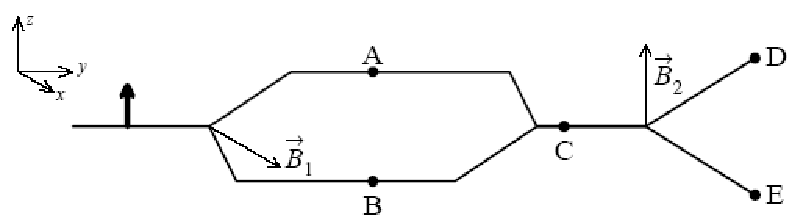
\includegraphics{graphics/SpinREXMQ2005.pdf}
\caption{Mesure du spin 1/2}
\label{fig:MesureSpinEx2011}
\end{figure}

On considérera que le faisceau $A$, tout comme le faisceau $D$ des questions
\ref{Q:q3}. et \ref{Q:q4}. ci-dessous, a la plus grande valeur du spin.

\begin{enumerate}
\item  Donner dans la base $\{\ket{+}_{z},\ket{-}_{z}\}$, la matrice de
l'opérateur $\mathtt{R}_{y}(\theta)$ de rotation d'angle $\theta$ autour de $Oy$
d'un spin $\frac{1}{2}$.

\item Expliquer clairement pourquoi on obtient deux faisceaux à la sortie de
SG1, en donnant l'état du spin en $A$ et $B$ et les probabilités de détection
$\mathcal{P}_{A}$ et $\mathcal{P}_{B}$.

\item\label{Q:q3} On enlève les détecteurs $A$ et $B$ précédents, et les deux
faisceaux sont recombinés en un seul faisceau avant de pénétrer à nouveau dans
un deuxième appareil de Stern-Gerlach, SG2, orienté selon $Oz$. A la sortie de
SG2, on place deux détecteurs $D$ et $E$.

Quel est l'état de spin des quantons détectés en $D$ et $E$ et quelles sont les
probabilités $\mathcal{P}_{D}$ et $\mathcal{P}_{E}$?

\item\label{Q:q4}On place un absorbeur en $A$, c'est-à-dire que SG1 agit comme
un filtre qui ne laisse passer que le faisceau $B$.

Quel est l'état de spin des quantons détectés en $D$ et $E$ et quelles sont les
probabilités $\mathcal{P}_{D}$ et $\mathcal{P}_{E}$? Considérer en particulier
le cas de $\theta=\frac{\pi}{2}$.

\item Quelles commentaires pouvez-vous faire par rapport aux probabilités
obtenues aux questions \ref{Q:q3}. et \ref{Q:q4}.?
\end{enumerate}

